% ************************************************************************
%
% Automated neuron tracing using probability hypothesis density filtering
%
% ************************************************************************
\chpos{15mm}{8mm}
\chapter[Automated neuron tracing using probability hypothesis density filtering]{Automated neuron tracing using probability hypothesis density filtering}
\chaptermark{Automated neuron tracing using PHD filtering}
\label{ch3:phd}
% abstract
{\small \lettrine{T}{he} functionality of neurons and their role in neuronal networks is tightly connected to the cell morphology. A fundamental problem in many neurobiological studies aiming to unravel this connection is the digital reconstruction of neuronal cell morphology from microscopic image data. Many methods have been developed for this, but they are far from perfect, and better methods are needed. In this chapter, a new method for tracing neuron centerlines needed for full reconstruction is presented. The method uses a fundamentally different approach than previous methods by considering neuron tracing as a Bayesian multi-object tracking problem. The problem is solved using probability hypothesis density filtering. Results of experiments on 2D and 3D fluorescence microscopy image datasets of real neurons indicate the proposed method performs comparably or even better than the state of the art.\par}
\vspace*{22em}
% ************************************************************************
\begin{publish}
	Based upon: M. Radojevi\'{c}, E. Meijering, ``Automated neuron tracing using probability hypothesis density filtering'', \textit{Bioinformatics}, vol. 33, no. 7, pp.1073-1080, 2017.   
\end{publish}

\section{Introduction}
\label{ch3:sec:introduction}
Accurate reconstruction of the tree-like structure of neuronal cells from optical microscopy images is a crucial step in automating the analysis of single neuron morphology or the connectivity of neuronal networks \cite{meijering2010neuron, donohue2011automated, peng2015bigneuron}. Microscopic images provide detailed information about the geometrical and topological properties of the neuronal arbors. Extracting and representing this information in a faithful and convenient digital format is key to many studies \cite{ascoli2002computational, ascoli2007neuromorpho, svoboda2011past, senft2011brief, halavi2012digital, lu2015quantitative}, as digital reconstructions enable neurobiologists to use computational approaches in addressing open issues in brain research, such as the relation between neuron structure and function, and the effects of neurodegenerative disease processes and drug compounds on neuron development and connectivity.

Existing approaches to tracing neurons in images can be broadly divided into global and local approaches. Global approaches consider the problem from the whole-image perspective and typically involve global image segmentation \cite{wearne2005new, basu2013segmentation, de2016graph} or global optimization strategies \cite{turetken2011automated, xiao2013app2}. Local approaches, on the other hand, use local image exploration strategies starting from seed points \cite{peng2011automatic, choromanska2012automatic, yang2013distance} to find segments of the neuronal tree, which are then merged into a full tree representation. Both approaches have advantages and disadvantages and they are often combined to profit from their complementarity \cite{zhao2011automated, jimenez2015improved}.

A wide variety of computational concepts have been proposed in developing automated neuron tracing methods, whether global or local \cite{acciai2016automated}. These include active contours \cite{cai2006repulsive, wang2011broadly, luo2015neuron}, tubular models \cite{santamaria2015automatic}, principal curves \cite{bas2011principal, quan2016neurogps}, perceptual grouping \cite{narayanaswamy20113}, path pruning \cite{peng2011automatic, xiao2013app2}, critical point detection \cite{al2008improved, radojevic2016fuzzy}, voxel scooping \cite{rodriguez2009three}, dynamic and integer programming \cite{zhang2007automated, turetken2012automated}, active learning \cite{gala2014active}, graph optimization \cite{turetken2011automated, chothani2011automated}, tubularity flow field segmentation \cite{mukherjee2015tubularity}, marked point processes \cite{basu2016neurite}, iterative back-tracking \cite{liu2016rivulet}, and more. A key characteristic relevant to the methodology presented in this chapter is that the vast majority of them are deterministic by nature. That is, they utilize models and algorithms that always assume or pass through the exact same sequence of states. While this behavior may seem virtuous and practically convenient, it is nonetheless not very realistic and not necessarily advantageous, for several reasons. For starters, expert human annotators, which are still considered to be the gold standard in evaluating methods, do not operate deterministically: their output will be (slightly) different every time they repeat a task. Also, any deterministic model is typically a (gross) simplification of reality, and consequently lacks flexibility in dealing with data variability. Finally, since every run of a deterministic algorithm will yield exactly the same output, it is not possible to accumulate evidence from multiple iterations. 

In this chapter, a new method for neuron tracing in optical microscopy images is proposed that operates probabilistically rather than deterministically. Focusing on delineating the branch centerlines, it utilizes a Bayesian approach to blend two sources of information: the model (based on prior knowledge) and the measurements (from the image data). The main novelty is that it combines the problems of neuron segment detection and linking into one framework by performing simultaneous multi-object tracking. Traditional multi-object (also referred to as multi-target) tracking techniques \cite{mahler2007statistical, stone2013bayesian} typically assume the number of objects to be known and/or they explicitly associate measurements with objects which are then Bayesian filtered individually \cite{bar1995multitarget}. In arbor tracing, the number of objects (neuron segments) is unknown a priori, therefore a different approach is used, based on filtering the so-called probability hypothesis density (\gls{phd}) function \cite{mahler2003multitarget}. PHD filtering has gained popularity in recent years as a robust approach to tracking, since it is able to compensate for missing detections and to remove noise and clutter, while reducing the computational complexity from exponential to linear as the number of objects grows. Applications include radar and sonar tracking \cite{tobias2005probability, clark2007particle}, video surveillance \cite{maggio2008efficient, wang2008data}, and even motion tracking in microscopy \cite{wood2012simplified, schlangen2016marker}, but had not been explored for neuron tracing yet. Moreover, presented application differs fundamentally from other works in the sense that the filtering is applied in space rather than in time.  The proposed method is evaluated on a variety of real image data (both 2D and 3D) taking expert manual annotations as the gold standard. Its performance is also compared with several state-of-the-art tools for neuron tracing \cite{chothani2011automated, xiao2013app2, quan2016neurogps}.

\section{Methods}
\label{ch3:sec:methods}
\subsection{Multi-object Bayesian filtering} 
\label{ch3:ssec:multi-obj-bay-filt}
Single-object tracking is considered as a Bayesian inference problem \cite{bar2004estimation, sarkka2013bayesian}. The key idea is to estimate the posterior probability density function (pdf) $f_{k|k}(\mathrm{x}_k | \mathrm{z}_{1:k})$, where $\mathrm{x}_k$ denotes the object state at iteration $k$, and $\mathrm{z}_{1:k}$ the sequence of observations from iterations $1$ to $k$ inclusive. Estimation is accomplished by sequentially applying prior knowledge to predict the state in the next iteration and updating this estimate with available observations. Similarly, multi-object tracking can be formulated as the problem of updating predictions of the multi-object state $\mathrm{X}_k = \{\mathrm{x}_{k,1},\ldots,\mathrm{x}_{k,N_k}\}$ with multi-object observations $\mathrm{Z}_k = \{\mathrm{z}_{k,1},\ldots,\mathrm{z}_{k,M_k}\}$, where $N_k$ and $M_k$ denote the number of objects and observations at iteration $k$, respectively. The prediction is thus formulated as:
\begin{equation}
f_{k|k-1}(\mathrm{X}_k | \mathrm{Z}_{1:k-1}) = 
\int\!\mathrm{\Pi}_{k|k-1}(\mathrm{X}_k | \mathrm{X}_{k-1}) f_{k-1|k-1}(\mathrm{X}_{k-1}|\mathrm{Z}_{1:k-1}) \delta\mathrm{X}_{k-1}
\label{ch3:eq:prediction}
\end{equation}
along with the update:
\begin{equation}
f_{k|k}(\mathrm{X}_k|\mathrm{Z}_{1:k}) =
\frac{\vartheta_k(\mathrm{Z}_k|\mathrm{X}_k) f_{k|k-1}(\mathrm{X}_k|\mathrm{Z}_{1:k-1})}{\int\!\vartheta_k(\mathrm{Z}_k|\mathrm{X})f_{k|k-1}(\mathrm{X}|\mathrm{Z}_{1:k-1}) \delta\mathrm{X}}\qquad\qquad
\label{ch3:eq:update}
\end{equation}
where $\mathrm{\Pi}_{k|k-1}(\mathrm{X}_k | \mathrm{X}_{k-1})$ denotes the multi-object state transition probability and $\vartheta_k(\mathrm{Z}_k|\mathrm{X}_k)$ the multi-object likelihood. Filtering the multi-object posterior $f_{k|k}(\mathrm{X}_k | \mathrm{Z}_{1:k})$ suffers from serious practical obstacles, as the multi-object state can be very high-dimensional and hard to sample and integrate efficiently. Moreover, it is necessary to take into account changes in object numbers, which adds an often intractable combinatorial burden. Thus more feasible solutions are needed.
\begin{figure}
	\centering
	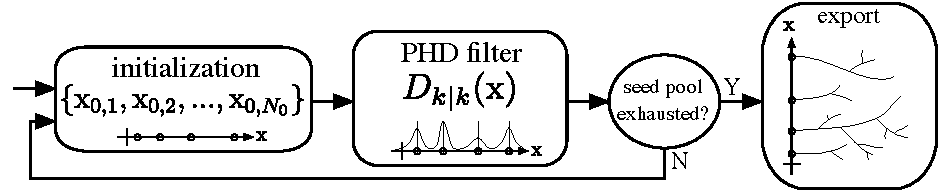
\includegraphics[width=0.8\linewidth]{fig1}
	\caption{Method overview. Each multi-object filtering round is initialized with $N_0$ seeds. If the seed pool is not exhausted by the end of the current round, a new round is started, and this is repeated until all seeds have been processed.}
	\label{ch3_fig1}
\end{figure}
\subsection{Probability hypothesis density filtering}
\label{ch3:ssec:prob-hyp-den}
To overcome the difficulties of direct multi-object Bayesian filtering, presented solution proposes instead to filter the first-order statistical moment of the multi-object posterior $f_{k|k}(\mathrm{X}_{k}|\mathrm{Z}_{1:k})$, computed as
\begin{equation}
D_{k|k}(\mathrm{x}|\mathrm{Z}_{1:k}) = \int\!\delta_{\mathrm{X}}(\mathrm{x})f_{k|k}(\mathrm{X}|\mathrm{Z}_{1:k})\delta\mathrm{X}
\label{eq:Dkk}
\end{equation}
where $\delta_{\mathrm{X}}$ denotes the sum of Dirac deltas at elements of $\mathrm{X}$. For the sake of notational convenience the left-hand side of (\ref{eq:Dkk}) is abbreviated to $D_{k|k}(\mathrm{x})$ in the sequel. This function, known as the probability hypothesis density (PHD) \cite{mahler2003multitarget}, is a non-negative function whose integral $\int\!D_{k|k}(\mathrm{x})\mathrm{d}\mathrm{x}$ yields the expected number of objects $\nu_{k}\in\mathbb{R}$. PHD filtering allows for joint detection and estimation of an unknown and varying number of objects and their individual states using the Bayesian prediction and update framework. Here, multi-object state $\mathrm{X}_k$ and observation $\mathrm{Z}_k$ are modeled as so-called random finite sets \gls{rfs}, with randomness in set size as well as set element values \cite{bar1995multitarget}, accommodating phenomena such as object initiation, clutter, and partitioning (spawning). 

\begin{figure}
	\centering
	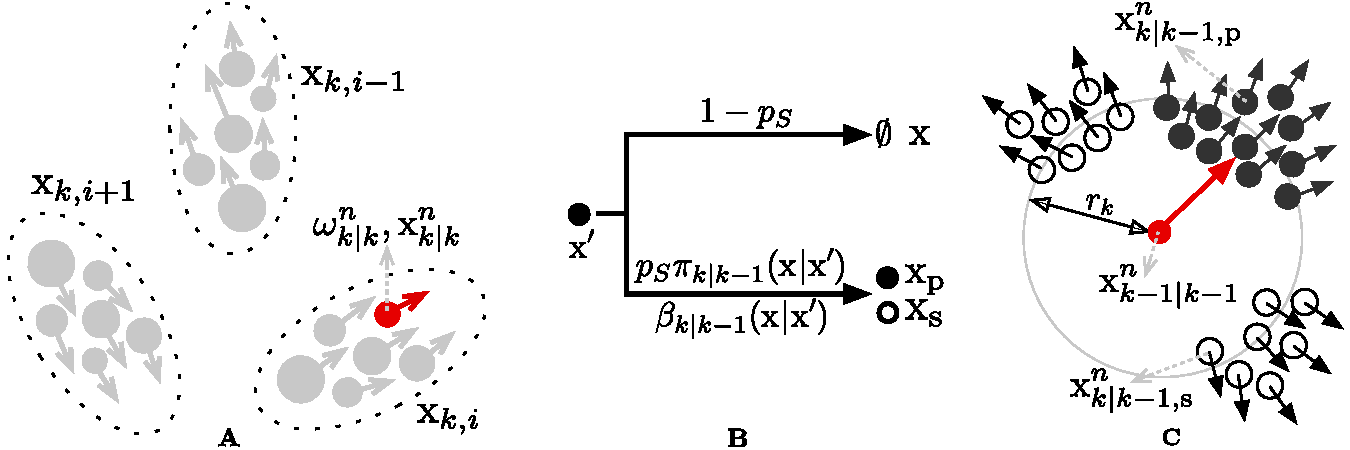
\includegraphics[width=.9\linewidth]{fig2}
	\caption{PHD filtering using a particle representation. (A) Each object $i$ at iteration $k$ has a state $\mathrm{x}_{k,i}$ that is represented by random particles $\mathrm{x}_{k|k}^{n}$ with corresponding weights $\omega_{k|k}^{n}$. (B) In the transition from iteration $k-1$ to $k$ an object ($\mathrm{x}'$) may disappear ($\emptyset$), persist ($\mathrm{x}_{\mathrm{p}}$), or spawn ($\mathrm{x}_{\mathrm{s}}$) according to the corresponding transition functions. Here $p_S$ is shorthand notation for $p_{S,k|k-1}(\mathrm{x}')$, since in practice a constant is used (Table~\ref{ch3:tab:params}). (C) For each particle a prediction $\mathrm{x}_{k-1|k-1}^n \rightarrow \mathrm{x}_{k|k-1}^n$ is made within radius $r_k$ according to the transition functions for persistence (p) and spawning (s).}
	\label{ch3_fig2}
\end{figure}
Formally stated, PHD filtering proceeds by iterating the sequence consisting of the prediction, formulated as
\begin{equation}
D_{k|k-1}(\mathrm{x}) = \gamma_{k|k-1}(\mathrm{x})\ + 
\langle \beta_{k|k-1}(\mathrm{x}|\cdot) + p_{S,k|k-1}(\cdot)\pi_{k|k-1}(\mathrm{x}|\cdot),D_{k-1|k-1}(\cdot) \rangle
\label{eq:phd-pred}
\end{equation}
followed by the update, formulated as
\begin{equation}
D_{k|k}(\mathrm{x}) = (1-p_{D,k}(\mathrm{x})) D_{k|k-1}(\mathrm{x})\ +
\sum\limits_{\mathrm{z}\in\mathrm{Z}_k}\!\frac{p_{D,k}(\mathrm{x})g_k(\mathrm{z}|\mathrm{x}) D_{k|k-1}(\mathrm{x}) }{C_k(\mathrm{z})+\langle p_{D,k}(\cdot)g_k(\mathrm{z}|\cdot),D_{k|k-1}(\cdot) \rangle}
\label{eq:phd-update}
\end{equation}
where $\gamma_{k|k-1}$ denotes the intensity function of newborn objects from iteration $k-1$ to $k$, $\beta_{k|k-1}$ the spawning object transition density, $p_{S,k|k-1}$ the object survival probability, $\pi_{k|k-1}$ the single-object transition density, $p_{D,k}$ the object detection probability, $g_k$ the single-object likelihood, $C_k$ the clutter intensity function, and $\langle g(\cdot),f(\cdot) \rangle \equiv \int\!f(\xi)g(\xi)\mathrm{d}\xi$ (see e.g.\ \cite{vo2006gaussian} for details). An analytical solution to (\ref{eq:phd-pred})-(\ref{eq:phd-update}) is provided by the Gaussian-mixture PHD (GM-PHD) filter \cite{vo2006gaussian} but it is based on linear Gaussian assumptions regarding object birth and dynamics. A more general solution is offered by sequential Monte-Carlo PHD (SMC-PHD) filtering \cite{vo2005sequential, ristic2010improved, zajic2003particle}, which approximates the PHD with a set of $N$ random particles $\mathrm{x}_{k|k}^{n}$ and corresponding weights $\omega_{k|k}^{n}$ as
\begin{equation}
\label{eq:smc-approx}
D_{k|k}(\mathrm{x}) \approx \sum\limits_{n=1}^{N} \omega_{k|k}^{n} \delta_{\mathrm{x}_{k|k}^{n}}\!(\mathrm{x})
\end{equation}
so that the classic particle filtering scheme \cite{doucet2000sequential, arulampalam2002tutorial, ristic2004beyond} can be applied.

\subsection{PHD-filtering based neuron tracing}
\label{ssec:proposed-neur-trac-meth}
\subsubsection{Definition and initialization}
\label{sssec:initialization}
The multi-object filtering scheme proposed for neuron tracing defines the object state as an oriented location:
\begin{equation}
\mathrm{x} = \left[ \mathrm{p}_{\mathrm{x}}, \mathrm{v}_{\mathrm{x}} \right] = \left[x, y, z, v_x, v_y, v_z\right] 
\label{eq:obj-state}
\end{equation}
where $\mathrm{p}_{\mathrm{x}}=[x, y, z]$ denotes the location and $\mathrm{v}_{\mathrm{x}}=[v_x, v_y, v_z]$ the local orientation of a tubular segment. Filtering starts from a set of $N_0$ seeds (Fig.~\ref{ch3_fig1}) sampled from a seed pool consisting of the local maxima of the tubularity image $\tau(x,y,z)$ computed from the original image using Hessian-based multiscale line filtering \cite{sato1998three} and min-max normalized to $[0,1]$. Local maxima are sorted in descending order so that seeds with high tubularity (meaning high confidence in the underlying image structure being a neuron branch) are processed first. To avoid seeds being selected too close together, in other words to ensure good spatial coverage of the neuron with seeds, for each selected seed (while going from top to bottom of the sorted list) the seeds within a circular neighborhood with radius $r_0$ are ignored in the current round. If, after SMC-PHD filtering (described in following Sec.~\ref{ssec:smc-phd-rec}), the seed pool is not exhausted, a new round is started by selecting a new set of seeds. During filtering, the observation consists of the location and corresponding tubularity value:
\begin{equation}
\mathrm{z} = \left[ \mathrm{p}_{\mathrm{z}}, \tau_{\mathrm{z}} \right] = \left[x, y, z, \tau\right]
\label{eq:observation}
\end{equation}
\subsubsection{SMC-PHD algorithm}
\label{ssec:smc-phd-rec}
The proposed method implements neuron tracing by SMC-PHD filtering. It is based on an approximation of $D_{k|k}(\mathrm{x})$ in (\ref{eq:smc-approx}) using $N=\rho N_k$ particles, where $N_k$ denotes the number of objects to be filtered, and $\rho$ the number of particles per object. That is, the state of object $i$ at iteration $k$, denoted $\mathrm{x}_{k,i}$, is represented by $\rho$ random particles $\mathrm{x}_{k|k}^{n}$ with corresponding weights $\omega_{k|k}^{n}$ (Fig.~\ref{ch3_fig2}A). The multi-object state transition in the prediction step (\ref{eq:phd-pred}) is a collection of single-object transitions (Fig.~\ref{ch3_fig2}B) that are approximated with transitions at the particle level (Fig.~\ref{ch3_fig2}C). More specifically, at the initial iteration $k=0$, $N_0$ seeds are selected and $\rho$ particles are sampled in a circular neighborhood with radius $r_0$ around each seed location using the tubularity value for importance sampling to determine the weights, resulting in the weighted particle set $\lbrace \omega_{0|0}^n, \mathrm{x}_{0|0}^n \rbrace_{n=1}^{\rho N_0}$. The initial local orientation of each particle, $\mathrm{v}_{\mathrm{x}_{0|0}^n}$, is the unit vector pointing from the seed location to the particle location $\mathrm{p}_{\mathrm{x}_{0|0}^n}$. Subsequently, the prediction (\ref{eq:phd-pred}) and update (\ref{eq:phd-update}) steps are executed for iterations $k=1,2,3,\dots$, until convergence. The transition and observation models (described next) allow to incorporate application-specific knowledge in this process. At iteration $k$, the set of weighted particles $\lbrace \omega_{k-1|k-1}^n, \mathrm{x}_{k-1|k-1}^n \rbrace_{n=1}^{\rho N_{k-1}}$ from iteration $k-1$ is used to predict $\eta$ new particles for each persistent and spawned object (Fig.~\ref{ch3_fig2}C). In the update step (\ref{eq:phd-update}), a set of observations $\lbrace \mathrm{z}_{k,j}\rbrace_{j=1}^{M_k}$ is used to update the predicted particle weights, followed by estimation of the states $\lbrace \hat{\mathrm{x}}_{k,i}\rbrace_{i=1}^{N_k}$. The detailed algorithm pseudo code of the introduced neuron tracing method is presented in Alg.~\ref{alg:delin}.
\begin{algorithm}
	\caption{Neuron tracing}\label{alg:delin}
	\begin{algorithmic}[1]
		\State{}{$k=0$}\Comment{Initialize}
		\State{}{$\lbrace \omega_{0|0}^n, \mathrm{x}_{0|0}^n \rbrace_{n=1}^{\rho N_0}$}\Comment{Initial particle and observation set}
		\State{}{$\lbrace \hat{\mathrm{x}}_{0,i} \rbrace_{i=1}^{N_{0}}$}\Comment{Initial estimate}
		\Repeat
		\State{}{$k=k+1$}
		\State{}{$\mathrm{p}_{i}^{n} \sim h(\mathrm{p} | \hat{\mathrm{x}}_{k-1,i}) \quad n \in \left[ 1, \rho N_{k-1}\right]$}\Comment{Draw observation particles} \label{alg:line:draw-obs-particles} 
		\State{}{$\mathrm{p}_{i,j}^n \in \mathscr{C}_j , \quad j \in \left[ 1, M_k \right], \quad n \in \left[ 1, |\mathscr{C}_j| \right]$}\Comment{Cluster observation particles}
		\State{}{$\mathrm{z}_{k,j} = \left[ \mathrm{p}_{i,j}^{\hat{n}}, \tau(\mathrm{p}_{i,j}^{\hat{n}}) \right]$}\Comment{Select representative sample} \label{alg:line:construct-obs} 
		\State{}{$\mathrm{Z}_{k} = \lbrace \mathrm{z}_{k,j},\dots, \mathrm{z}_{k,M_k}  \rbrace$}\Comment{Construct observations}
		\State{}{$\lbrace \omega_{k|k}^n, \mathrm{x}_{k|k}^n \rbrace_{n=1}^{\rho N_{k}}, \nu_{k}, \lbrace \hat{\mathrm{x}}_{k,i} \rbrace_{i=1}^{N_k} \leftarrow$ SMC-PHD$(\lbrace \omega_{k-1|k-1}^n, \mathrm{x}_{k-1|k-1}^n \rbrace_{n=1}^{\rho N_{k-1}}, \mathrm{Z}_{k})$}\Comment{Algorithm~\ref{alg:smc-phd}}
		\Until{$\left[ \nu_{k} \right] = 0$} \Comment{$\left[ \cdot \right] \equiv $ nearest integer}
	\end{algorithmic}
\end{algorithm}
\subsubsection{Transition model}
\label{sssec:prediction-model}
In the prediction step (\ref{eq:phd-pred}), three types of objects are assumed: newborn, persisting, and spawned objects \cite{vo2005sequential,vo2006gaussian}. By design, newborn objects are not considered in presented tracing algorithm, since the seeding is used, hence $\gamma_{k|k-1}(\mathrm{x})=0$.

Persisting objects in the current iteration correspond directly to existing objects in the previous iteration. In algorithm, the transition density for predicting persistent object $\mathrm{x}$ given object $\mathrm{x'}$ in the previous iteration, is calculated as
\begin{equation}
\label{eq:persist-prediction}
\pi_{k|k-1}(\mathrm{x}|\mathrm{x'}; \kappa, r_k) = \frac{1}{\tilde{\pi}} e^{\frac{-(\vert \mathrm{p}_{\mathrm{x}} - \mathrm{p}_{\mathrm{x'}}  \vert - r_k)^2  }{2 (r_k/3)^2}} \frac{e^{\kappa (\mathrm{v}_{\mathrm{x}} \cdot \mathrm{v}_{\mathrm{x'}})}}{2 \pi I_0(\kappa)}
\end{equation}
where $\tilde{\pi}$ is a normalization factor such that the sum of $\pi_{k|k-1}$ over $\vert \mathrm{p}_{\mathrm{x}} - \mathrm{p}_{\mathrm{x'}} \vert \leq 2r_k$ is unity, and $I_0$ is the zero-order Bessel function of the first kind. The first factor corresponds to a radial profile that peaks at the prediction step size $r_k$. The second factor is a circular normal distribution (von Mises) parametrized with the unit direction vector $\mathrm{v}_{\mathrm{x'}}$ from the previous iteration and circular variance $\kappa$. Here, $\mathrm{v}_{\mathrm{x}} = (\mathrm{p}_{\mathrm{x}} - \mathrm{p}_{\mathrm{x'}})/\vert \mathrm{p}_{\mathrm{x}} - \mathrm{p}_{\mathrm{x'}} \vert$, which connects the predicted location $\mathrm{p}_{\mathrm{x}}$ with the location $\mathrm{p}_{\mathrm{x'}}$ from the previous iteration. Particles $\mathrm{x}_{k|k-1,\mathrm{p}}^{n}$ (Fig.~\ref{ch3_fig2}C) are drawn using $\pi_{k|k-1}$ as importance sampling function.

A spawned object is a new instance derived (spawned) from an existing object in the previous iteration. This allows dealing with bifurcations during tracing. In the showcased algorithm, the transition density for predicting a spawned object $\mathrm{x}$ given $\mathrm{x'}$ in the previous iteration, is calculated as
\begin{equation}
\label{eq:spawn-prediction}
\beta_{k|k-1}(\mathrm{x}|\mathrm{x'}; \kappa, r_k) = \frac{1}{\tilde{\beta}} e^{\frac{-(\vert \mathrm{p}_{\mathrm{x}} - \mathrm{p}_{\mathrm{x'}} \vert-r_k)^2}{2(r_k/3)^2}} \cdot \prod\limits_{i=0}^{1} \left( 1 - \frac{e^{\kappa (-1^i \mathrm{v}_{\mathrm{x}} \cdot \mathrm{v}_{\mathrm{x'}})}}{2 \pi I_0(\kappa)} \right)
\end{equation}
where $\tilde{\beta}$ is a normalization factor such that the sum of $\beta_{k|k-1}$ over $\vert \mathrm{p}_{\mathrm{x}} - \mathrm{p}_{\mathrm{x'}} \vert \leq 2r_k$ is unity. 
\begin{figure}
	\centering
	\begin{tabular}{c@{\hspace{1em}}c@{\hspace{1em}}c}
		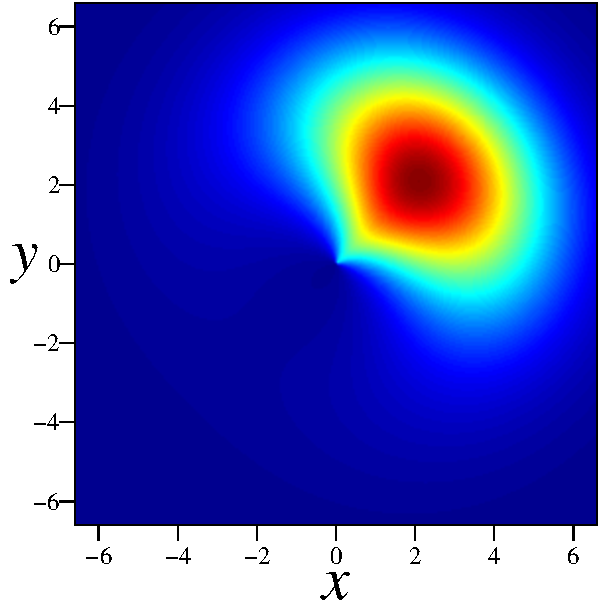
\includegraphics[height=0.3\columnwidth]{fig3a_embedded} &
		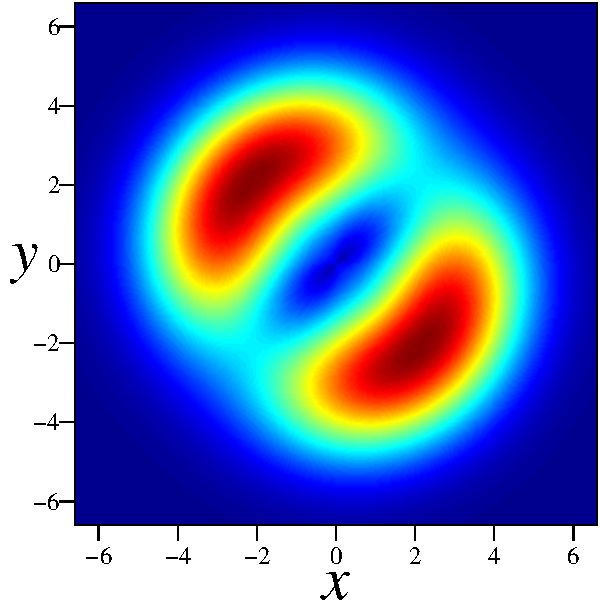
\includegraphics[height=0.3\columnwidth]{fig3b_embedded} &
		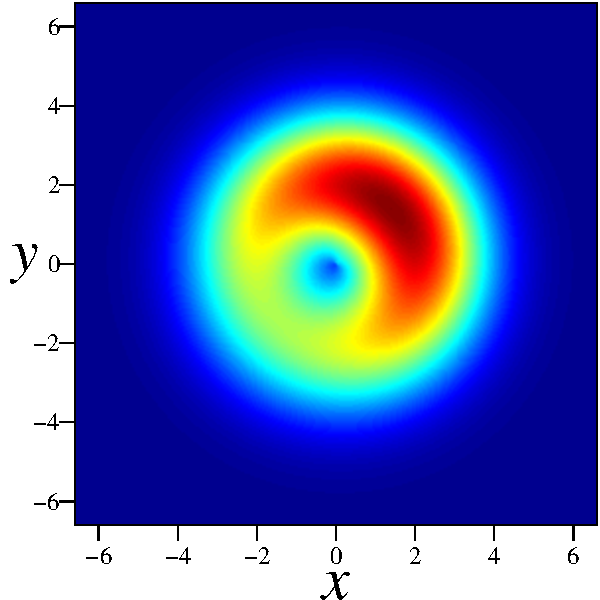
\includegraphics[height=0.3\columnwidth]{fig3c_embedded} \\
		a) $\pi_{k|k-1}(\mathrm{x}|\mathrm{x'})$ & b) $\beta_{k|k-1}(\mathrm{x}|\mathrm{x'})$ & c) $h(\mathrm{p}|\mathrm{x'})$ \\
	\end{tabular}  		
	\caption{Transition densities (2D examples) for persistent a) and spawned b) objects with $z=0$, $\mathrm{x'}=\left[ 0,0,0, \tfrac{1}{\sqrt{2}},\tfrac{1}{\sqrt{2}}, 0 \right] $, $\kappa=2$, and $r_k=3$. c) Importance sampling used in the observation model without the tubularity component, $\tau(\mathrm{p})=1$, and $\kappa=0.5$. Rainbow color coding is used running from blue (indicating low values) to red (indicating high values).}
	\label{ch3_fig3}
\end{figure}
The first factor has the same form as in (\ref{eq:persist-prediction}) and the second factor is the aggregate of the complementary circular normal distributions used for spawning objects in positive and negative direction. An example of the intensity profile of $\pi_{k|k-1}$ and $\beta_{k|k-1}$ is shown in Fig.~\ref{ch3_fig3}. Particles $\mathrm{x}_{k|k-1,\mathrm{s}}^{n}$ (Fig.~\ref{ch3_fig2}C) are drawn using $\beta_{k|k-1}$ as importance sampling function.

\subsubsection{Observation model}
\label{sssec:observation-model}
In the update step (\ref{eq:phd-update}), a set of observations $\{\mathrm{z}_{k,j}\}_{j=1}^{M_k}$ is used to update the predictions from (\ref{eq:phd-pred}). Observations have a corrective role as they carry information about the neuron centerline locations and corresponding tubularity values (\ref{eq:observation}). The importance sampling function $h$
\begin{equation}
\label{eq:observation-importance-sampling}
h(\mathrm{p} | \mathrm{x'}; \kappa, r_k) = \frac{1}{\tilde{h}} e^{\frac{ -(\vert \mathrm{p} - \mathrm{p}_{\mathrm{x'}}  \vert - r_k)^2  }{2 (r_k/3)^2}} \frac{e^{\kappa (\mathrm{v}_{\mathrm{p}} \cdot \mathrm{v}_{\mathrm{x'}})}}{2 \pi I_0(\kappa)} \tau(\mathrm{p})
\end{equation}%as the importance sampling function 
is used to obtain the observations, where $\tilde{h}$ is a normalization factor such that the sum of $h$ over $\vert \mathrm{p} - \mathrm{p}_{\mathrm{x'}} \vert \leq 2r_k$ is unity, and $\mathrm{v}_{\mathrm{p}}=(\mathrm{p}-\mathrm{p}_{\mathrm{x'}})/\vert \mathrm{p}-\mathrm{p}_{\mathrm{x'}}\vert$. The first two factors have the same form as in (\ref{eq:persist-prediction}) but here $\kappa$ is typically lower to make the update step more restrictive than the prediction step. The third factor is the normalized tubularity measure $\tau$ \cite{sato1998three} at location $\mathrm{p}$, which makes the observations correspond preferably to regions with high tubularity, which are indeed more likely to contain neuron structures.

To obtain the observations at iteration $k$, for each object $i$ from the previous iteration a set of particles $\{\mathrm{p}_{i}^{n}\}_{n=1}^{\rho N_{k-1}}$ is drawn from $h$ using $\mathrm{x'}=\hat{\mathrm{x}}_{k-1,i}$ (the object state estimate), with particle weight proportional to the tubularity value at that location. All these particles together are subsequently clustered in an unsupervised manner using mean-shifting \cite{cheng1995mean}, resulting in a set of clusters $\lbrace \mathscr{C}_j \rbrace_{j=1}^{M_k}$, with each cluster $\mathscr{C}_j$ having a subset $\lbrace\mathrm{p}_{i,j}^n\rbrace_{n=1}^{|\mathscr{C}_j|}$ of the particles. For each cluster, a representative sample $\mathrm{p}_{i,j}^{\hat{n}}$ is calculated using least-squares optimization,
\begin{equation}
\label{eq:n-measure} % \setminus \lbrace n \rbrace
\hat{n} = \argmin_n \!\!\!\!\!\sum\limits_{m \in \left[ 1, |\mathscr{C}_j| \right]}\!\!\!\!\! \theta(\mathrm{p}_{i,j}^m, \mathrm{p}_{\hat{\mathrm{x}}_{k-1,i}}, \mathrm{p}_{i,j}^n)
\end{equation}
where $\theta(\mathrm{p}_0, \mathrm{p}_1, \mathrm{p}_2)$ denotes the squared Euclidean distance from point $\mathrm{p}_0$ to the line segment defined by $\mathrm{p}_1$ and $\mathrm{p}_2$, calculated as
\begin{multline}
\label{eq:theta}
\theta(\mathrm{p}_0, \mathrm{p}_1, \mathrm{p}_2) = \\
\begin{cases}
\vert \mathrm{p}_0 - \mathrm{p}_1 \vert^2 & \textrm{if\ } (\mathrm{p}_0-\mathrm{p}_1) \cdot (\mathrm{p}_2-\mathrm{p}_1) \leq 0 \\
\vert \mathrm{p}_0 - \mathrm{p}_2 \vert^2 & \textrm{if\ } (\mathrm{p}_0-\mathrm{p}_2) \cdot (\mathrm{p}_1-\mathrm{p}_2) \leq 0 \\
\frac{\vert(\mathrm{p}_2-\mathrm{p}_1) \times (\mathrm{p}_1-\mathrm{p}_0)\vert^2}{\vert\mathrm{p}_2-\mathrm{p}_1\vert^2} & \textrm{otherwise}
\end{cases}
\end{multline}
so that the line segment that best fits the cluster elements determines the selected location. From this the observation is obtained as $\mathrm{z}_{k,j} = [\mathrm{p}_{i,j}^{\hat{n}}, \tau(\mathrm{p}_{i,j}^{\hat{n}})]$. The process is illustrated in Fig.~\ref{ch3_fig4}.
\begin{figure}
	\centering
	\begin{tabular}{c@{\hspace{2em}}c}
		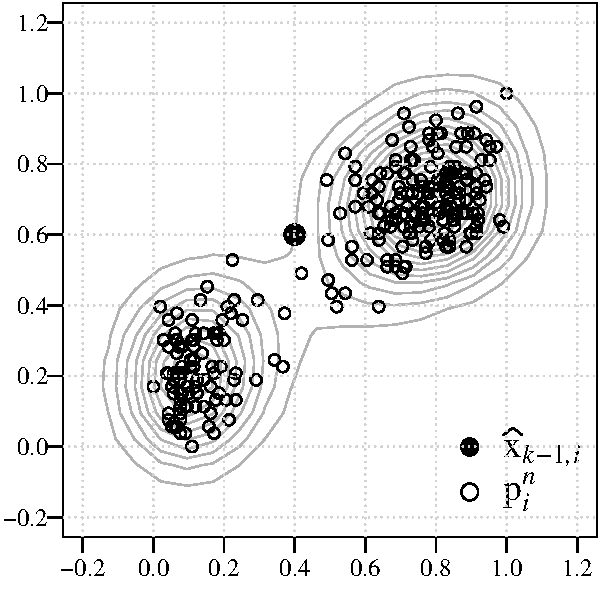
\includegraphics[width=0.4\columnwidth]{fig4a_embedded} &
		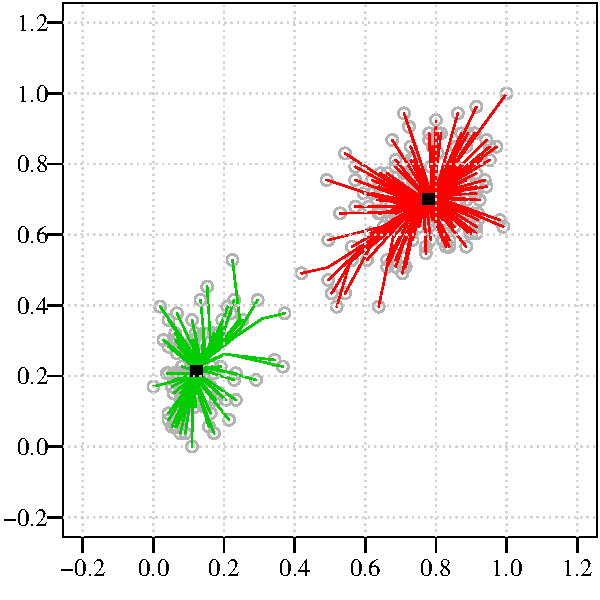
\includegraphics[width=0.4\columnwidth]{fig4b_embedded} \\[-1ex]
		a) $\mathrm{p}_{i}^{n} \sim h(\mathrm{p} | \hat{\mathrm{x}}_{k-1,i})$ &
		b) $\mathrm{p}_{i,j}^n \in \mathscr{C}_j$ \\[3ex]
		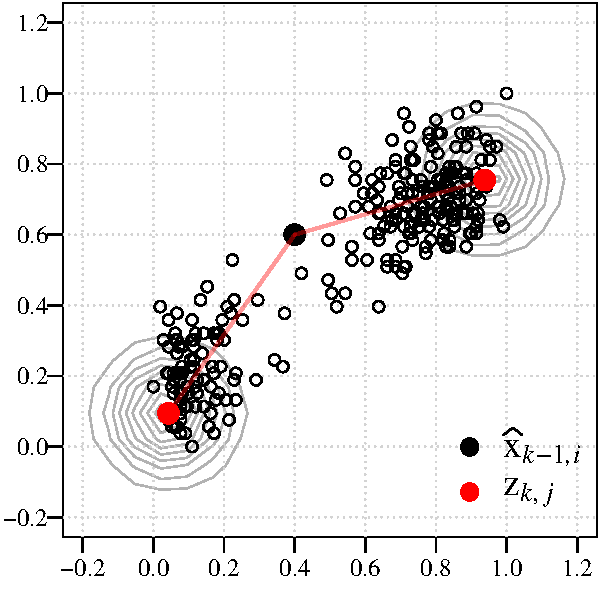
\includegraphics[width=0.4\columnwidth]{fig4c_embedded} &
		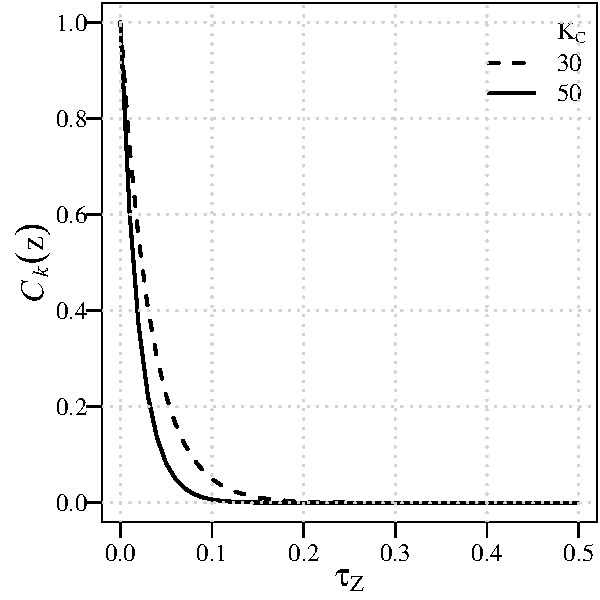
\includegraphics[width=0.4\columnwidth]{fig4d_embedded} \\[-1ex]
		c) $\mathrm{z}_{k,j}$ &
		d) $C_k(\mathrm{z}) = e^{-K_c\tau_{\mathrm{z}}}$ 
	\end{tabular}
	\caption{Formation of the observations (2D example). a) For each object $i$ from iteration $k-1$, particles $\mathrm{p}_{i}^{n}$ are sampled from the importance sampling function $h$, using the state estimate $\hat{\mathrm{x}}_{k-1,i}$. The solid dot indicates the location of $\hat{\mathrm{x}}_{k-1,i}$ and the contours represent lines of equal particle weight. (B) The particles are processed by mean-shifting resulting in clusters $\mathscr{C}_j$ whose labeled particles are denoted as $\mathrm{p}_{i,j}^{n}$. (C) Each observation $\mathrm{z}_{k,j}$ is obtained from the representative cluster particle $\mathrm{p}_{i,j}^{\hat{n}}$ as described in the main text. Contours represent lines of equal observation likelihood. (D) The clutter intensity function.} 
	\label{ch3_fig4}
\end{figure}
For the single-object likelihood in Eq.~\ref{eq:phd-update} a Gaussian function centered at the spatial location of the observation is used, $g_k(\mathrm{z}|\mathrm{x})=\exp(-\vert\mathrm{p}_{\mathrm{z}}-\mathrm{p}_{\mathrm{x}}\vert^2/2\sigma_{\mathrm{z}}^2)$, giving more importance to predictions closer to $\mathrm{z}$. The clutter intensity function is defined as an exponential dependency on the observation tubularity value, $C_k(\mathrm{z})=\exp(-K_{c}\tau_{\mathrm{z}})$, implying that the clutter increases as the tubularity value goes to zero. In practice, clutter plays a role in detecting terminal points, causing tracings with low particle weights (due to their proximity to regions with low tubularity values) to not be resampled and thus dropped after the update step.
\begin{algorithm}
	\caption{SMC-PHD filtering}\label{alg:smc-phd}
	\begin{algorithmic}[1]
		\State{Input:}{$\lbrace ( \omega_{k-1|k-1}^n, \mathrm{x}_{k-1|k-1}^n ) \rbrace_{n=1}^{\rho N_{k-1}}, \lbrace \mathrm{z}_{k,j}  \rbrace_{j=1}^{M_k}$}
		\Comment{$D_{k-1}(\mathrm{x})$ approx. observation $\mathrm{Z}_k$}
		\For{$n=1,\dots,\rho N_{k-1}$} 
		\For{$m=1,\dots,\eta$}
		\State{}{$i = (n-1)\eta+m$}
		\State{Draw: }{$\mathrm{x}_{k|k-1,\mathrm{p}} \sim \pi_{k|k-1}(\mathrm{x}|\mathrm{x}_{k-1|k-1}^{n}) \rightarrow \mathrm{x}_{k|k-1,\mathrm{p}}^{i}$}\Comment{Persistent object particles} \label{alg:line:pred-p} 
		\State{Compute: }{$\omega_{k|k-1, \mathrm{p}}^{i} = p_S \tfrac{1}{\eta} \omega_{k-1|k-1}^{n}$}
		\State{Draw: }{$\mathrm{x}_{k|k-1,\mathrm{s}} \sim \beta_{k|k-1}(\mathrm{x}|\mathrm{x}_{k-1|k-1}^{n}) \rightarrow \mathrm{x}_{k|k-1,\mathrm{s}}^{i}$}\Comment{Spawning object particles} \label{alg:line:pred-s} 
		\State{Compute: }{$\omega_{k|k-1, \mathrm{s}}^{i} = p_S \tfrac{1}{\eta} \omega_{k-1|k-1}^{n}$}
		\EndFor
		\EndFor
		\State{$\lbrace(\omega_{k|k-1}^n, \mathrm{x}_{k|k-1}^n)\rbrace_{n=1}^{S_k} = \lbrace(\omega_{k|k-1,\mathrm{p}}^n, \mathrm{x}_{k|k-1,\mathrm{p}}^n)\rbrace_{n=1}^{\rho \eta N_{k-1}} \cup \lbrace(\omega_{k|k-1,\mathrm{s}}^n, \mathrm{x}_{k|k-1,\mathrm{s}}^n)\rbrace_{n=1}^{\rho \eta N_{k-1}}$}{} \Comment{Union of particle sets}
		\For{$n=1,\dots,S_k$} % \limits
		\State{Update: }{$\omega_{k|k}^n = (1-p_D)\omega_{k|k-1}^n+\sum\limits_{\mathrm{z} \in \mathrm{Z}_k}\tfrac{p_D g_k(\mathrm{z}|\mathrm{x}_{k|k-1}^n) \omega_{k|k-1}^n}{C_k(\mathrm{z}) + \sum_{n=1}^{S_k}p_D g_k(\mathrm{z}|\mathrm{x}_{k|k-1}^n)\omega_{k|k-1}^n }$}\label{alg:line:particle-update}
		\EndFor
		\State{}{$\nu_k = \sum\limits_{n=1}^{S_{k}} \omega_{k|k}^n$} \Comment{Cardinality calculation}
		%\State{}{$N_{k} = \rho$} \Comment{}
		\State{Estimate: }{$\hat{\mathrm{x}}_{k,i} \leftarrow \lbrace  \omega_{k|k}^n, \mathrm{x}_{k|k-1}^n  \rbrace_{n=1}^{S_k}$}\Comment{Mean-shift clustering}
		% $N_k$ times 
		\State{Resample: }{$N_k=\left[ \nu_k \right], \lbrace  \omega_{k|k}^n  , \mathrm{x}_{k|k-1}^n  \rbrace_{n=1}^{S_k} \rightarrow \lbrace \omega_{k|k}^n ,  \mathrm{x}_{k|k}^n\rbrace_{n=1}^{\rho N_k}, \omega_{k|k}^n = \nu_k / (\rho N_k) $\\} \Comment{Systematic resampling with $\rho$ particles per object}
	\end{algorithmic}
\end{algorithm}

\subsubsection{Implementation details}
\label{sssec:implementation-details}
Algorithms~\ref{alg:delin} and~\ref{alg:smc-phd} provide a step-by-step overview of the introduced PHD-filtering based neuron tracing method. For testing purposes the method was implemented in Java as a plugin for ImageJ \cite{abramoff2004image}. The method has several parameters for which default parameters are given in Table~\ref{ch3:tab:params}. Based on the acquired experience, most of them do not require extensive tuning and the default values were used for the showcased experiments. An important aspect of any SMC-based algorithm is to use a sufficient number of particles in the approximations. The conducted experiments indicate that values of 10-20 are sufficient for $\rho$ and $\eta$ since the objects of interest in neuron-related applications are approximately 1D structures in 3D space and therefore are easily covered. Higher values can lead to higher accuracy and precision but at proportionally higher computational cost. The most important parameters are the numbers of seeds $N_0$ and rounds (Fig.~\ref{ch3_fig2}) and in the experiments (described next) the performance of the presented algorithm was tested for different values of these parameters.

\begin{table}
	\small\centering
	\begin{tabular}{c@{\hspace{3em}}c@{\hspace{3em}}l}
		\hline
		Parameter & Default & Description \\
		\hline
		$K_c$ & 30 & Clutter intensity function decay \\
		$N_0$ & 20 & Number of seed points per round \\
		$p_D$ & 0.9 & Object detection probability \\
		$p_S$ & 0.9 & Object survival probability \\
		$r_k$ & 3 voxels & Radial estimation step size \\
		$\rho$ & $\geq 10$ & Number of particles per object \\
		$\eta$ & $\geq 10$ & Number of predictions per particle \\
		$\kappa$ & 2 & Circular variance in (\ref{eq:persist-prediction}) \& (\ref{eq:spawn-prediction}) \\
		& 0.5 & Circular variance in (\ref{eq:observation-importance-sampling}) \\
		\hline
	\end{tabular}
	\vspace{0.5\baselineskip}
	\caption{Parameters of the proposed method with their default values. In accompanying implementation constants values were used for the object detection probability $p_D=p_{D,k}$ and the object survival probability $p_S=p_{S,k|k-1}$.}
	\label{ch3:tab:params}
\end{table}

\section{Results}
\label{ch3:sec:results}
\subsection{Neuron data sets} 
\label{ch3:subsec:neuron-datasets}
For evaluating the performance of the proposed method for both 2D and 3D neuron tracing, three data sets (Fig.~\ref{ch3_fig5}) were used. All datasets consist of real neuron images acquired with fluorescence microscopy. Two data sets are 3D image stacks from the DIADEM challenge \cite{brown2011diadem}: neocortical layer-1 axons (NCL1A) with 16 image stacks and olfactory projection fibers (OPF) with 9 image stacks. The third data set (HCN) consists of 30 2D images of hippocampal neurons \cite{steiner2002overexpression}. Together the data sets show a good variety of image contrast and structural complexity. Further details about the images can be retreived from the corresponding, cited publications.
\begin{figure}
	\centering
	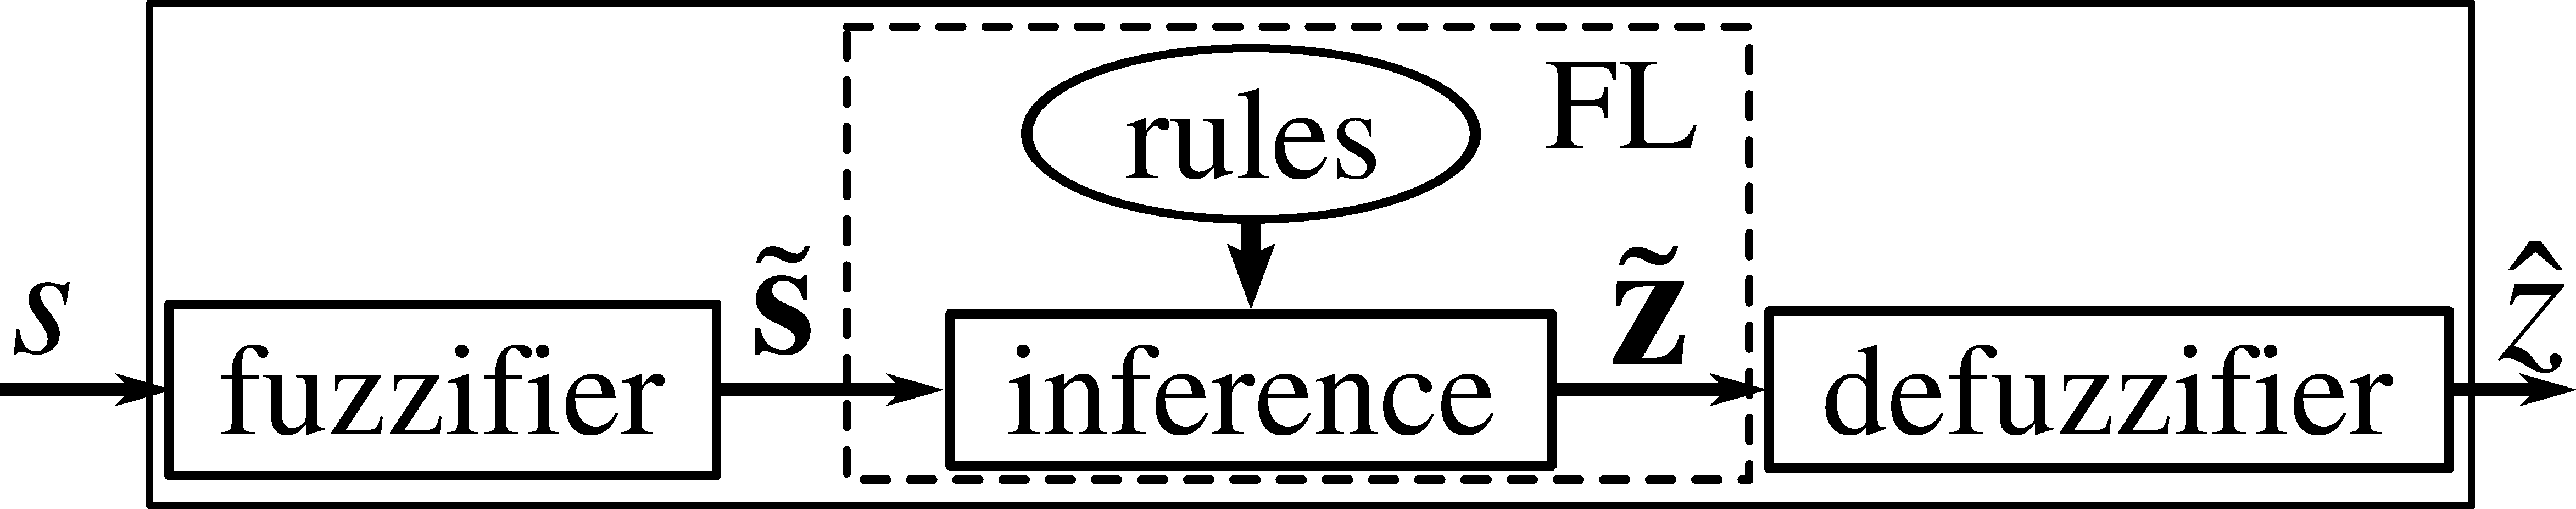
\includegraphics[width=\linewidth]{fig5}
	\caption{Example images with tracing results of the data sets used in the evaluation. Top row: NCL1A image stacks (volume rendered) showing a network of neocortical layer-1 axons. Middle row: OPF image stacks (volume rendered) showing olfactory projection fibers. Bottom row: HCN images showing hippocampal neurons. The tracings (overlaid in red) were obtained with the proposed method using 20 seeds and at most 10 rounds (up to 40 for the top row to capture more detail). For illustration purposes the image intensities are inverted in these visualizations compared to the originals, and the tracings are offset with respect to the neuron structures for better visual comparison.}
	\label{ch3_fig5}
\end{figure}
\subsection{Performance measures}
\label{subsec:performance-measures}
The accuracy of the tracings produced by the proposed method was assessed by comparison with the gold-standard obtained by manual delineation of the neuron structures \cite{gillette2011diademchallenge, meijering2004design}. To this end, two categories of evaluation measures are used. The first consists of measures summarizing the spatial Euclidean distances between the nodes of two tracings to be compared: the average spatial distance (SD), the average substantial spatial distance (SSD), and the fraction of nodes whose distance is at least the substantial distance (\%SSD). Similar to previous studies using these measures \cite{peng2010v3d}, the substantial distance was set to 2 (pixels in 2D and voxels in 3D). The second category of evaluation measures are based on the numbers of true-positive (TP), false-positive (FP), and false-negative (FN) nodes according to the substantial distance. From these, it is straightforward to compute the recall, $\textrm{R}=\textrm{TP}/(\textrm{TP}+\textrm{FN})$, and precision, $\textrm{P}=\textrm{TP}/(\textrm{TP}+\textrm{FP})$, summarized using the F-score, $\textrm{F}=2\,\textrm{P}\,\textrm{R}/(\textrm{P}+\textrm{R})$. Prior to computing these measures the tracings (from the method and the gold-standard) were resampled with an equal step size of 1 pixel using Vaa3D \cite{peng2010v3d}.

\begin{figure}
	\centering
	\begin{tabular}{c@{\hspace{1ex}}c@{\hspace{1ex}}c@{\hspace{3ex}}c@{\hspace{1ex}}c@{\hspace{1ex}}c}
		a) &
		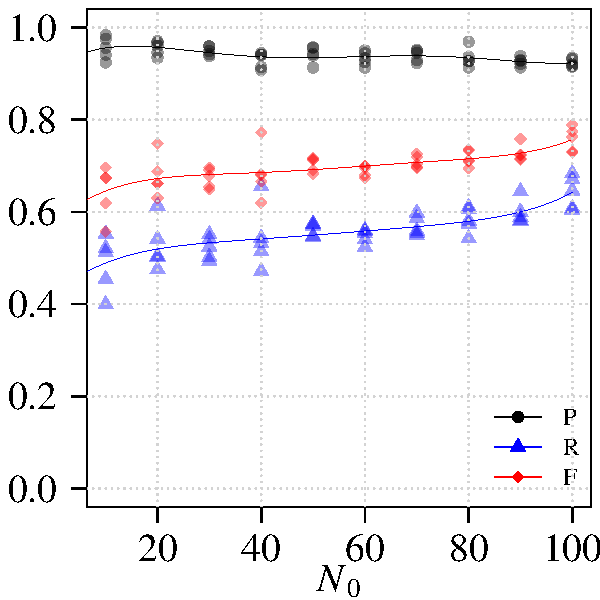
\includegraphics[align=c,width=0.2\columnwidth]{fig6a1_embedded} &
		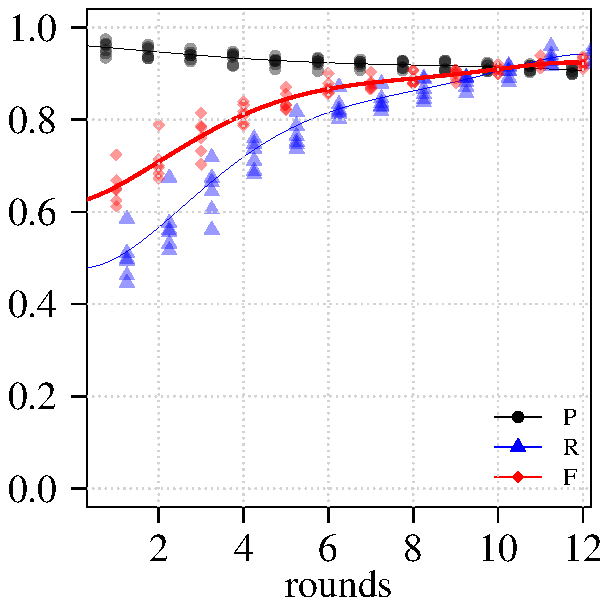
\includegraphics[align=c,width=0.2\columnwidth]{fig6a2_embedded} &
		b) &
		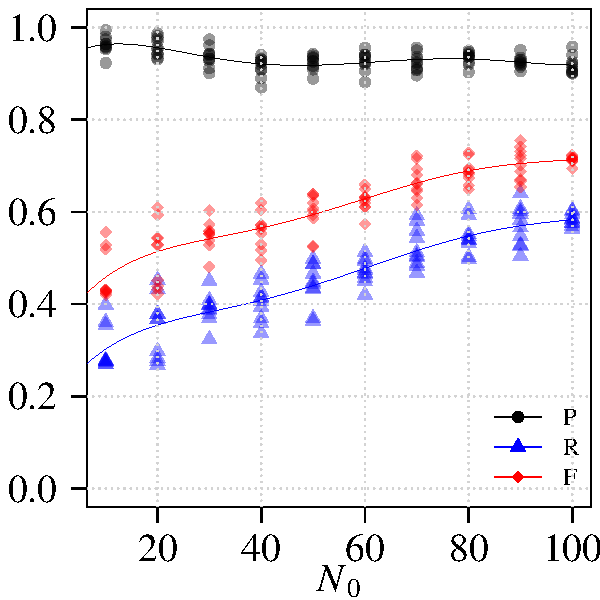
\includegraphics[align=c,width=0.2\columnwidth]{fig6b1_embedded} &
		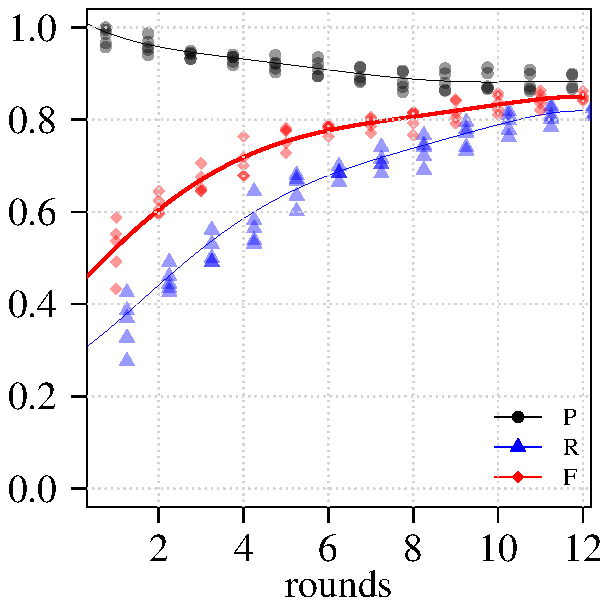
\includegraphics[align=c,width=0.2\columnwidth]{fig6b2_embedded} \\
		\vspace{-2ex} \\
		c) &
		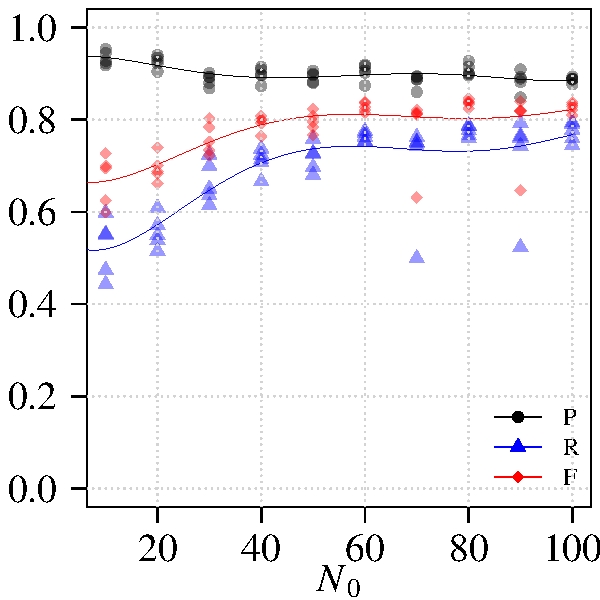
\includegraphics[align=c,width=0.2\columnwidth]{fig6c1_embedded} &
		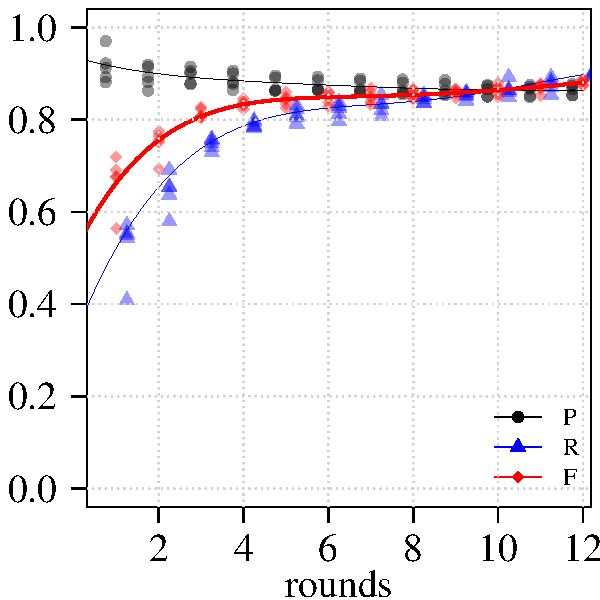
\includegraphics[align=c,width=0.2\columnwidth]{fig6c2_embedded} &
		d) &
		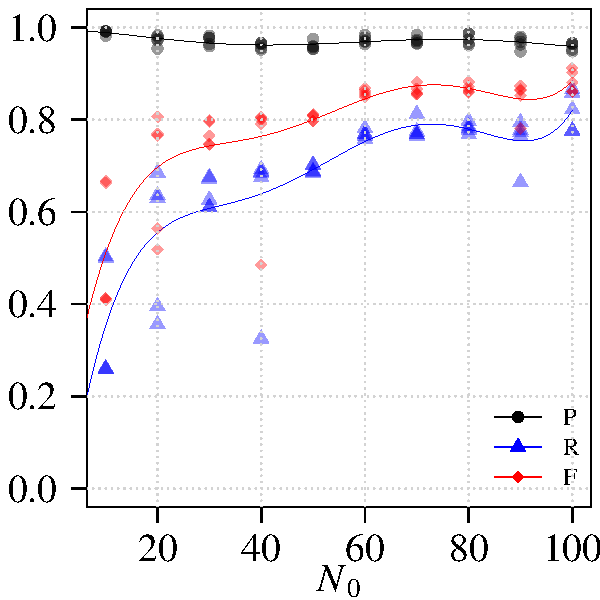
\includegraphics[align=c,width=0.2\columnwidth]{fig6d1_embedded} &
		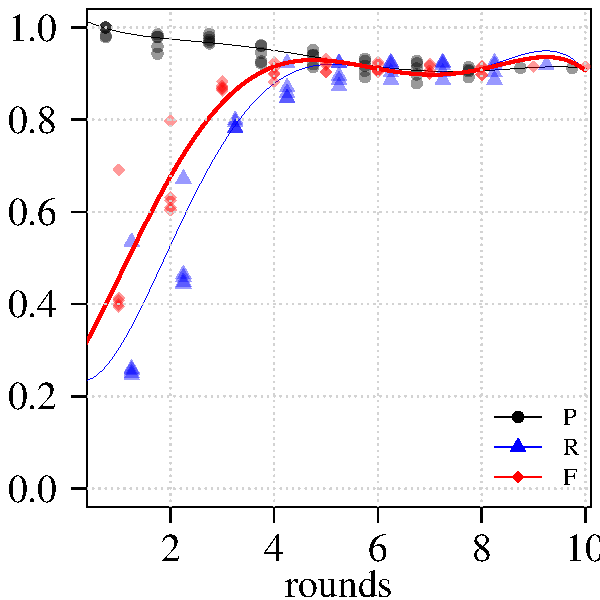
\includegraphics[align=c,width=0.2\columnwidth]{fig6d2_embedded} \\
		\vspace{-2ex} \\
		e) &
		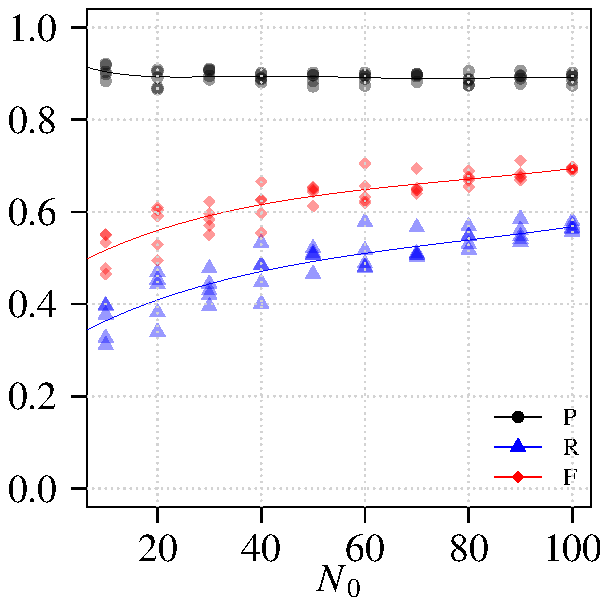
\includegraphics[align=c,width=0.2\columnwidth]{fig6e1_embedded} &
		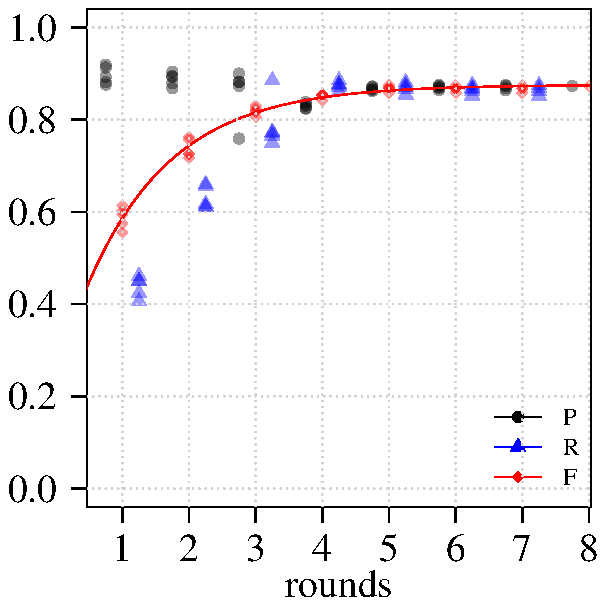
\includegraphics[align=c,width=0.2\columnwidth]{fig6e2_embedded} &
		f) &
		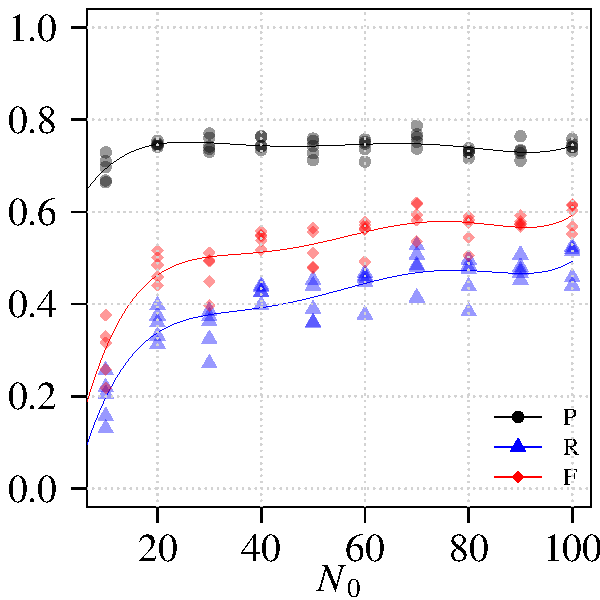
\includegraphics[align=c,width=0.2\columnwidth]{fig6f1_embedded} &
		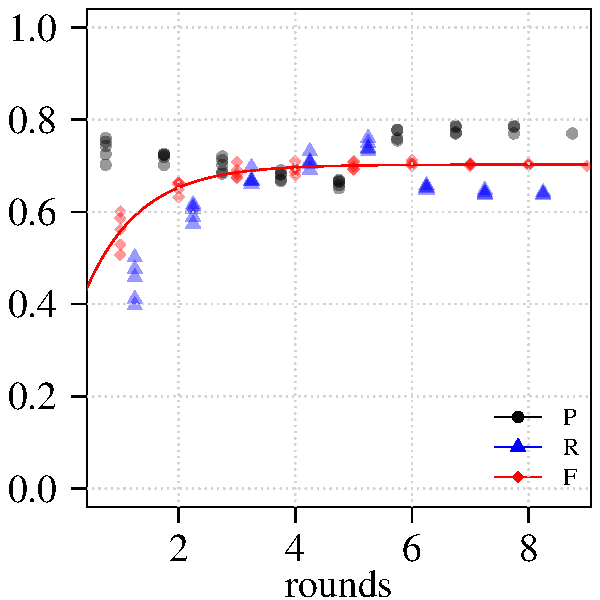
\includegraphics[align=c,width=0.2\columnwidth]{fig6f2_embedded} \\
		\vspace{-2ex} \\
		g) &
		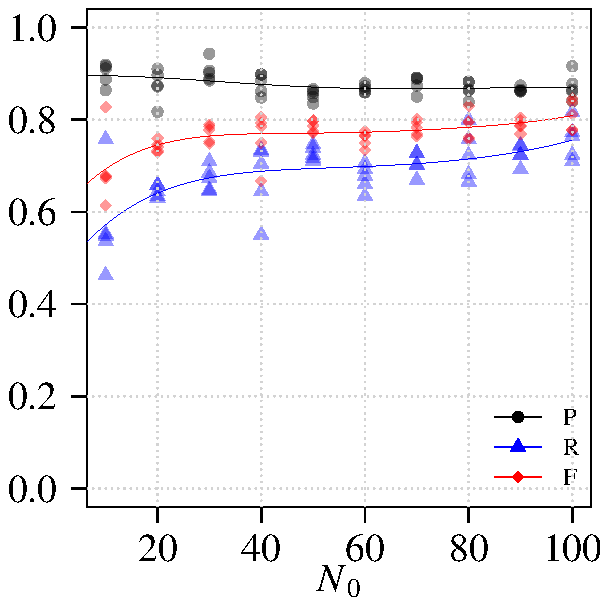
\includegraphics[align=c,width=0.2\columnwidth]{fig6g1_embedded} &
		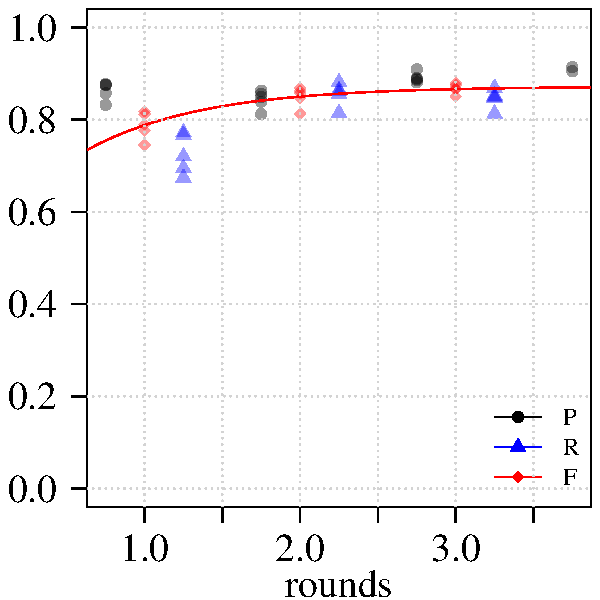
\includegraphics[align=c,width=0.2\columnwidth]{fig6g2_embedded} &
		h) &
		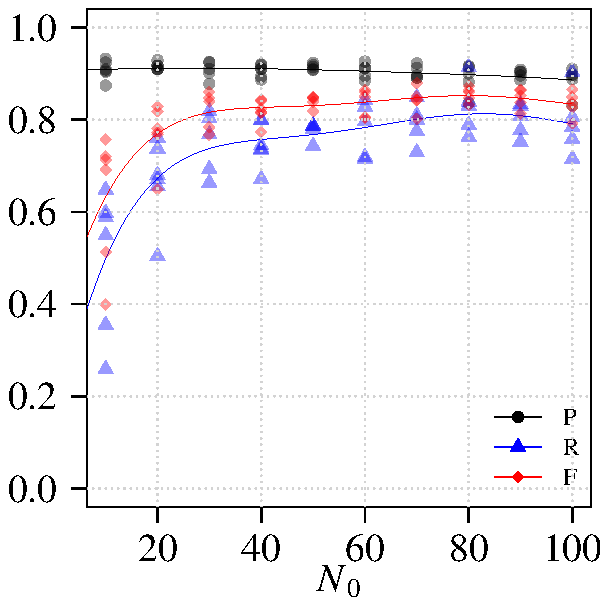
\includegraphics[align=c,width=0.2\columnwidth]{fig6h1_embedded} &
		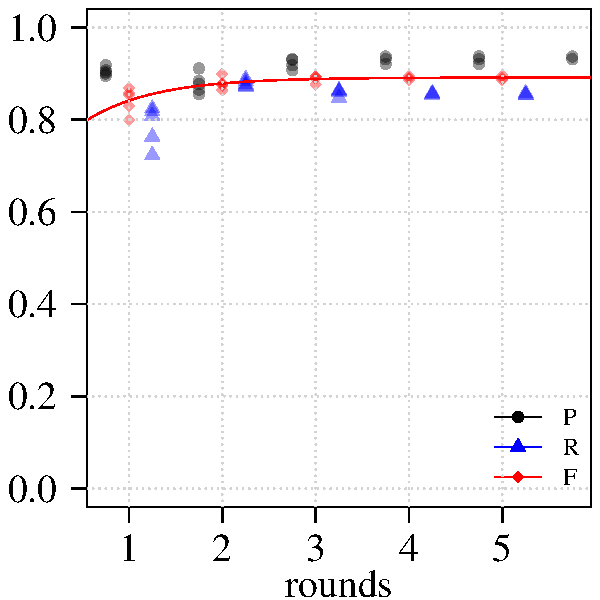
\includegraphics[align=c,width=0.2\columnwidth]{fig6h2_embedded} \\
	\end{tabular}
	\caption{Performance as a function of numbers of seeds and rounds for four example cases from the OPF (a-d) and the HCN (e-h) data set. Similar trends were observed for all cases in the respective data sets. Left panel per case: Precision (P), recall (R), and F-score (F) after one round initialized with different numbers of seeds ($N_0$). Right panel per case: The scores after multiple rounds with a fixed number of seeds ($N_0=40$). Fifth-order polynomial curves were fit to the data to show approximate trends.}
	\label{ch3_fig6}
\end{figure}

\subsection{Evaluation of method behavior} 
\label{subsec:evaluation-of-method-behavior}
First, behavior of the presented method was evaluated as a function of the number of seeds and rounds. For this experiment P, R, and F values were measured for 1) a single round of filtering with different numbers of seeds and 2) multiple rounds of filtering using a fixed number of seeds. Since the algorithm showcased in this chapter operates probabilistically, the results of five repetitions of the experiment were averaged. The results for the NCL1A data set are shown in Fig.~\ref{ch3_fig7} and for the other data sets in Fig.~\ref{ch3_fig6}. As expected, R and F generally increase, but P slightly decreases as the number of seeds and rounds increase, indicating an increase in the number of FP detections. The specific patterns may differ depending on the image content, but the observations indicate that as a function of the number of seeds, the increase of R and F levels off beyond about 40, therefore this value was subsequently used. As a function of the number of rounds, R and F level off after about 4 rounds, indicating there is no need in practice to run the method exhaustively on all possible seed points. This can be explained from the fact that seed selection proceeds from highest to lowest tubularity value, so that later seeds correspond to less and less valuable image structures, and the resulting tracings will be dropped due to low particle weights. Examples of traced neurons for the different data sets are shown in Fig.~\ref{ch3_fig5}. As can be observed from the examples in the top row of the figure, images with more fuzzy and fragmented structures may require more rounds to capture more detail. Alternatively, a better tubularity filter may be needed.

\begin{figure}[!b]
	\centering
	\begin{tabular}{c@{\hspace{0.05\linewidth}}c}
		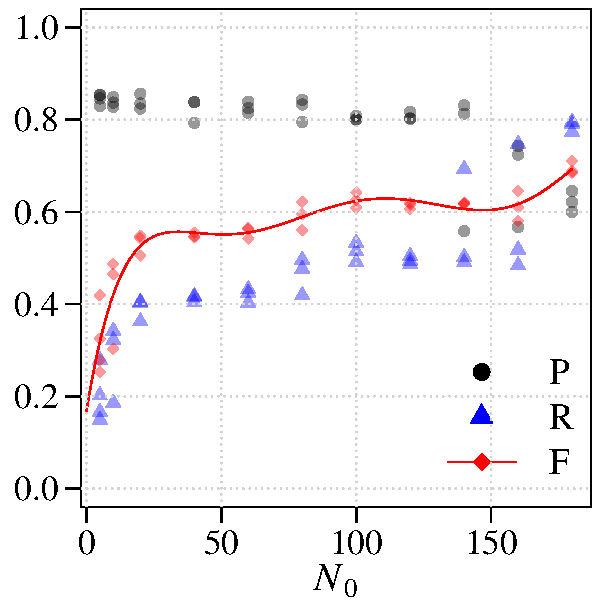
\includegraphics[width=0.45\linewidth]{fig7a_embedded} &
		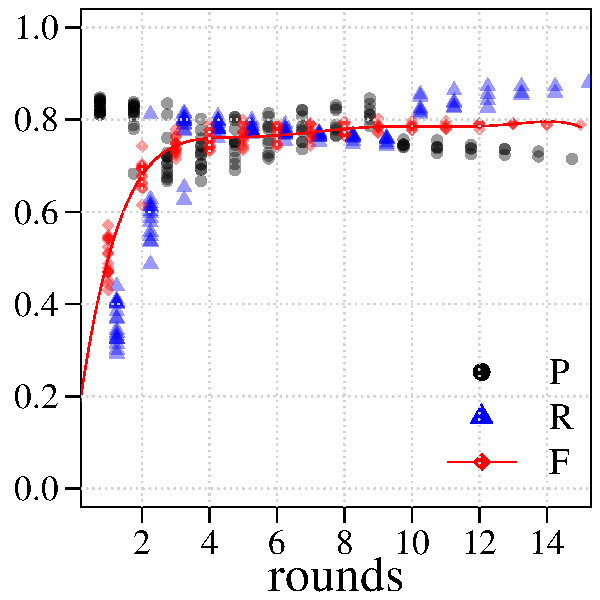
\includegraphics[width=0.45\linewidth]{fig7b_embedded} \\
	\end{tabular}
	\caption{Performance of the proposed method as a function of numbers of seeds and rounds for an example image stack from the NCL1A data set. Similar trends were observed for all stacks in the data set. Left panel: Precision (P), recall (R), and F-score (F) after one round initialized with different numbers of seeds ($N_0$). Right panel: The scores after multiple rounds with a fixed number of seeds ($N_0=40$). Fifth-order polynomial fitting was used to show the approximate F-score trend.}
	\label{ch3_fig7}
\end{figure}

\subsection{Comparison with other methods}
\label{subsec:comparison-with-other-methods}
Next the performance of the introduced method (PHD) was compared with several alterative methods, namely all-path pruning (APP2) \cite{xiao2013app2}, NeuroGPS-Tree (GPS) \cite{quan2016neurogps}, minimum spanning tree (MST) tracing as used in the BigNeuron project \cite{peng2015bigneuron}, and Neural Circuit Tracer (NCT) \cite{chothani2011automated}. For each of these methods the scores were optimized by trying all possible parameter values on a grid. The results for the NCL1A data set are shown in Fig.~\ref{ch3_fig12}, for the OPF data sets in Fig.~\ref{ch3_fig8} and HCN in Fig.~\ref{ch3_fig9}. Further observation shows that showcased method (results indicated in red) performs comparably or even better than the state-of-the-art methods. This suggests there may indeed be an advantage in using probabilistic approaches such as the one proposed in this work. It is also noticeable that NCT (results indicated in blue), while performing superiorly in most cases, required significant user interaction and manual correction to enable export of the tracings to the standard SWC file format used throughout the evaluations. Thus the results of this method include a high level of expert input and could serve as a reference. All other methods including the presented one were fully automatic after parameter selection.
\begin{figure}
	\centering
	\begin{tabular}{c@{\hspace{0.02\columnwidth}}c@{\hspace{0.02\columnwidth}}c}
		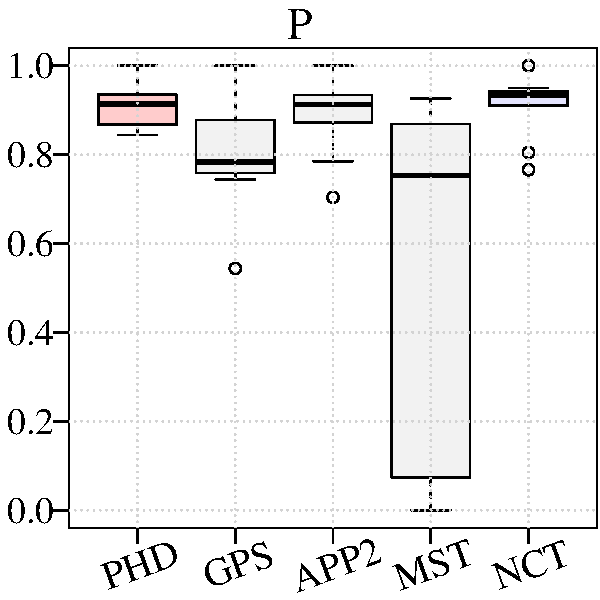
\includegraphics[width=0.31\columnwidth]{fig8a_embedded} &
		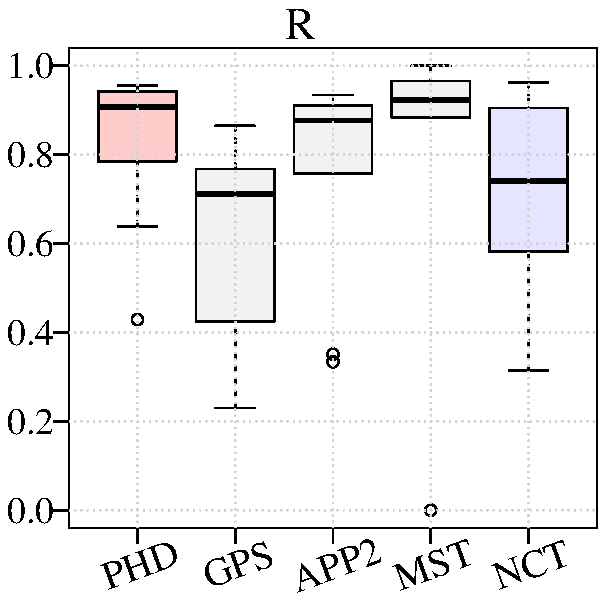
\includegraphics[width=0.31\columnwidth]{fig8b_embedded} &
		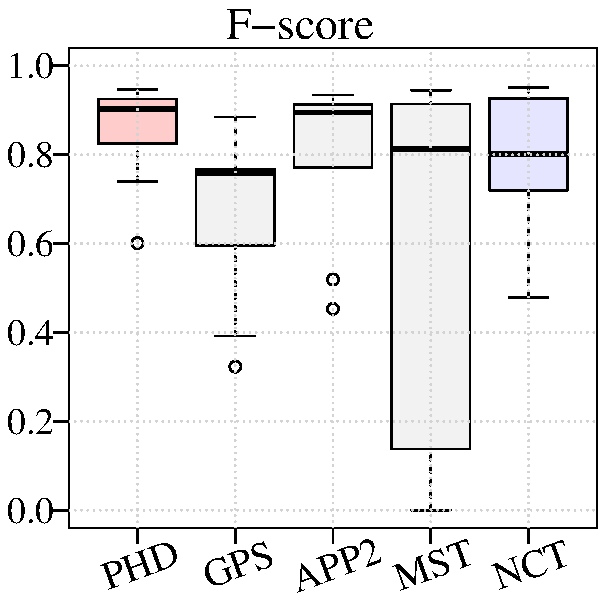
\includegraphics[width=0.31\columnwidth]{fig8c_embedded} \\
		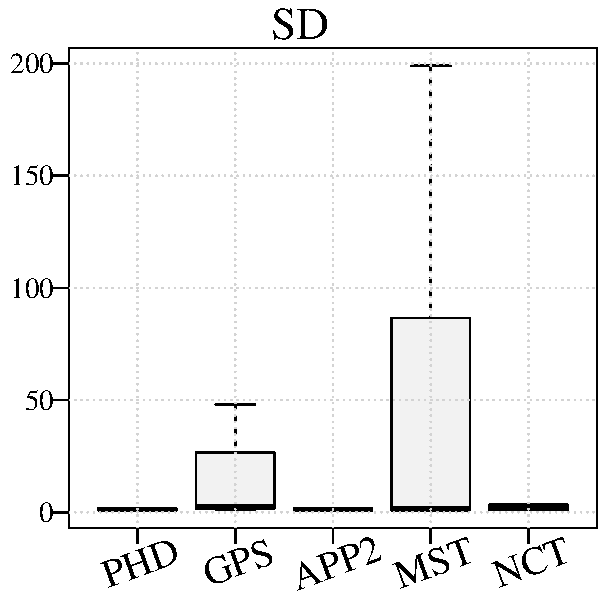
\includegraphics[width=0.31\columnwidth]{fig8d_embedded} &
		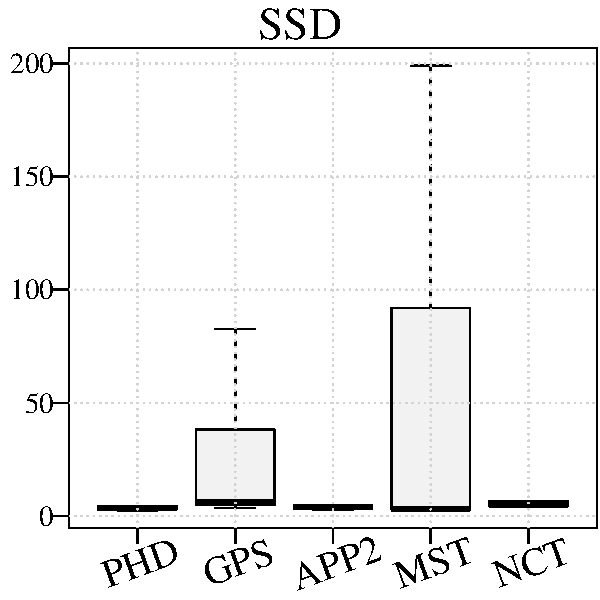
\includegraphics[width=0.31\columnwidth]{fig8e_embedded} &
		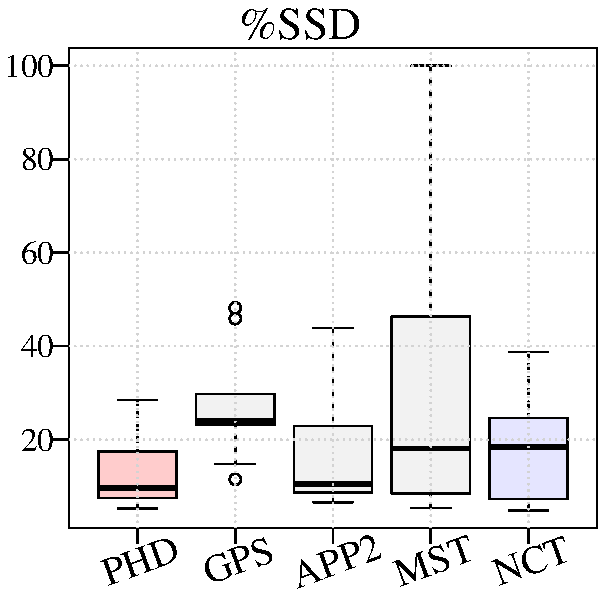
\includegraphics[width=0.31\columnwidth]{fig8f_embedded} \\
	\end{tabular}
	\caption{Performance comparison of the proposed method with several other methods on the OPF data set. For each method and each measure, the plotted box indicates the 25-75 percentile, the horizontal bar indicates the median score, and the whiskers and outliers are drawn using the default settings of R.}
	\label{ch3_fig8}
\end{figure}

\begin{figure}
	\centering
	\begin{tabular}{c@{\hspace{0.02\columnwidth}}c@{\hspace{0.02\columnwidth}}c}
		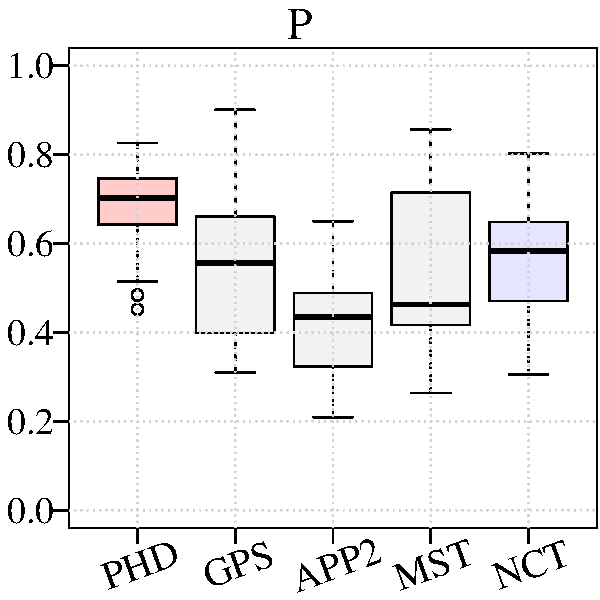
\includegraphics[width=0.31\columnwidth]{fig9a_embedded} &
		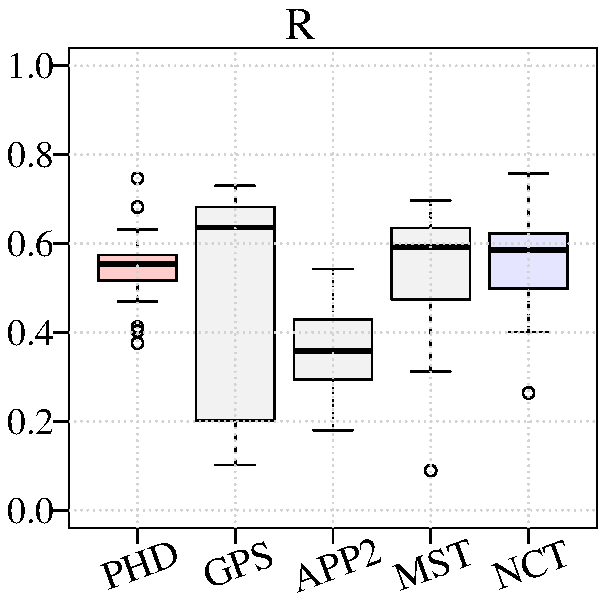
\includegraphics[width=0.31\columnwidth]{fig9b_embedded} &
		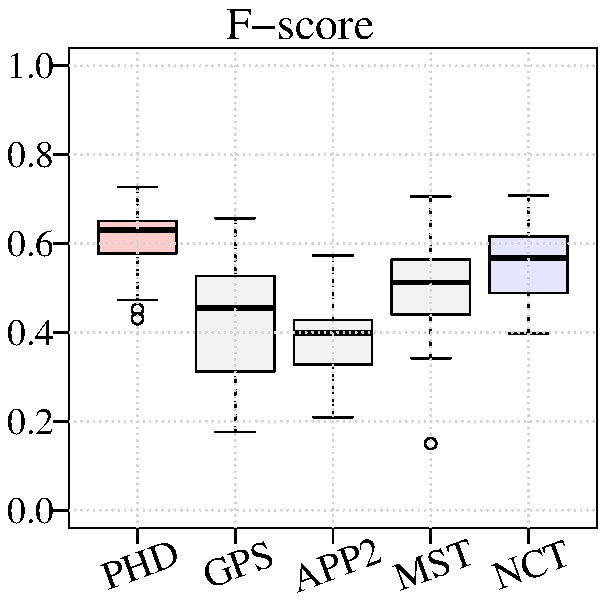
\includegraphics[width=0.31\columnwidth]{fig9c_embedded} \\
		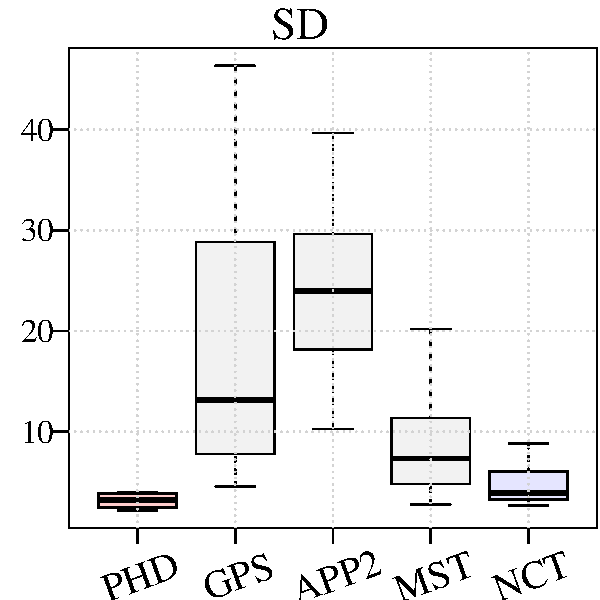
\includegraphics[width=0.31\columnwidth]{sd_saria_embedded} &
		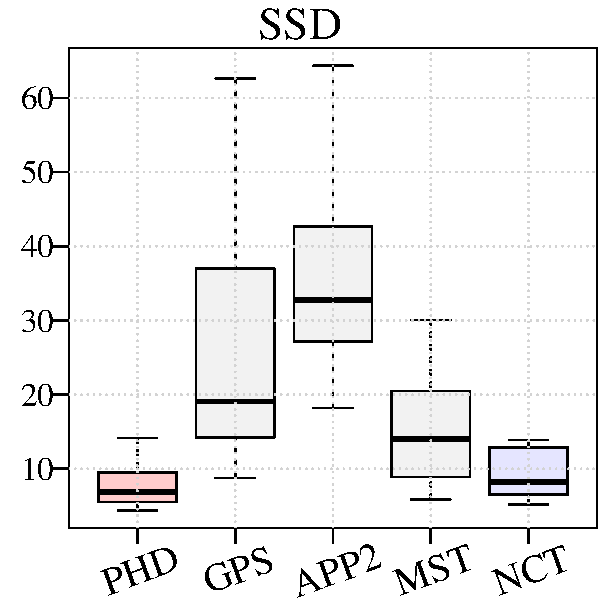
\includegraphics[width=0.31\columnwidth]{ssd_saria_embedded} &
		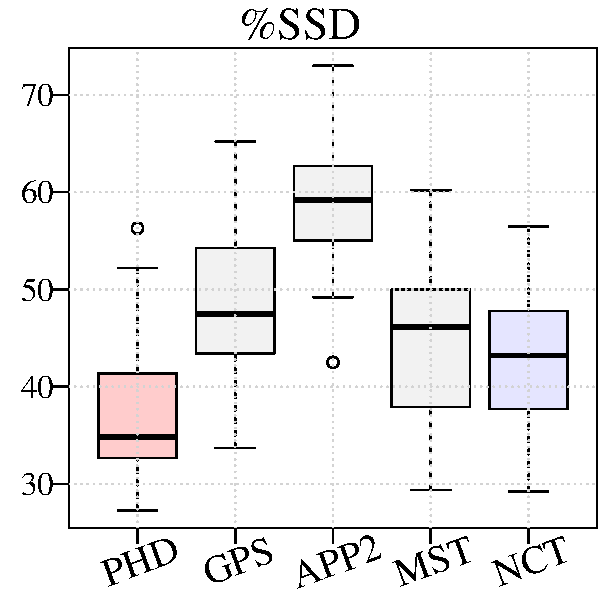
\includegraphics[width=0.31\columnwidth]{pssd_saria_embedded} \\
	\end{tabular}
	\caption{Performance comparison of the proposed method with several other methods on the HCN data set. For each method and each measure, the plotted box indicates the 25-75 percentile, the horizontal bar indicates the median score, and the whiskers and outliers are drawn using the default settings of R.}
	\label{ch3_fig9}
\end{figure}

To further demonstrate the advantage of the presented method over the others in challenging situations, the case when neuron fibers meet, run closely parallel to each other for some distance, and then diverge again was studied. In order to analyze the behavior of the different methods in a controlled manner, with increasing distance between the fibers, the images with two fibers of similar intensity and scale were synthesized. The results, shown in supplementary Fig.~\ref{ch3_fig10}, demonstrate that the method introduced in this chapter (PHD), similar to GPS, yields more faithful tracings than APP2 and MST. NCT was not included in these experiments for reasons mentioned above. Not surprisingly, all methods break down when the fibers overlap completely. In addition, even more challenging case was created, with three fibers of different intensity and scale. The results, shown in supplementary Fig.~\ref{ch3_fig11}, illustrate that the proposed method outperforms even the best alternatives.

\begin{figure}
	\centering
	\begin{tabular}{r@{\hspace{0.02\columnwidth}}c@{\hspace{0.02\columnwidth}}c@{\hspace{0.02\columnwidth}}c}
		Case: &
		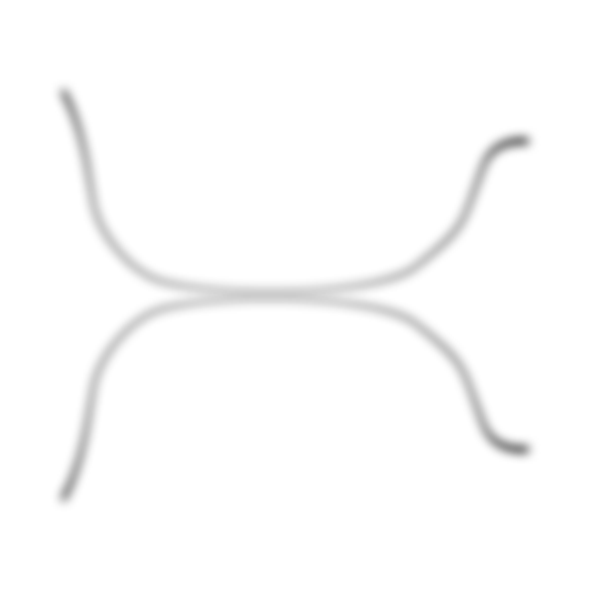
\includegraphics[align=c,width=0.15\columnwidth]{fig10a} &
		
\includegraphics[align=c,width=0.15\columnwidth]{fig10b} &
		
\includegraphics[align=c,width=0.15\columnwidth]{fig10c}\\
		PHD: &
		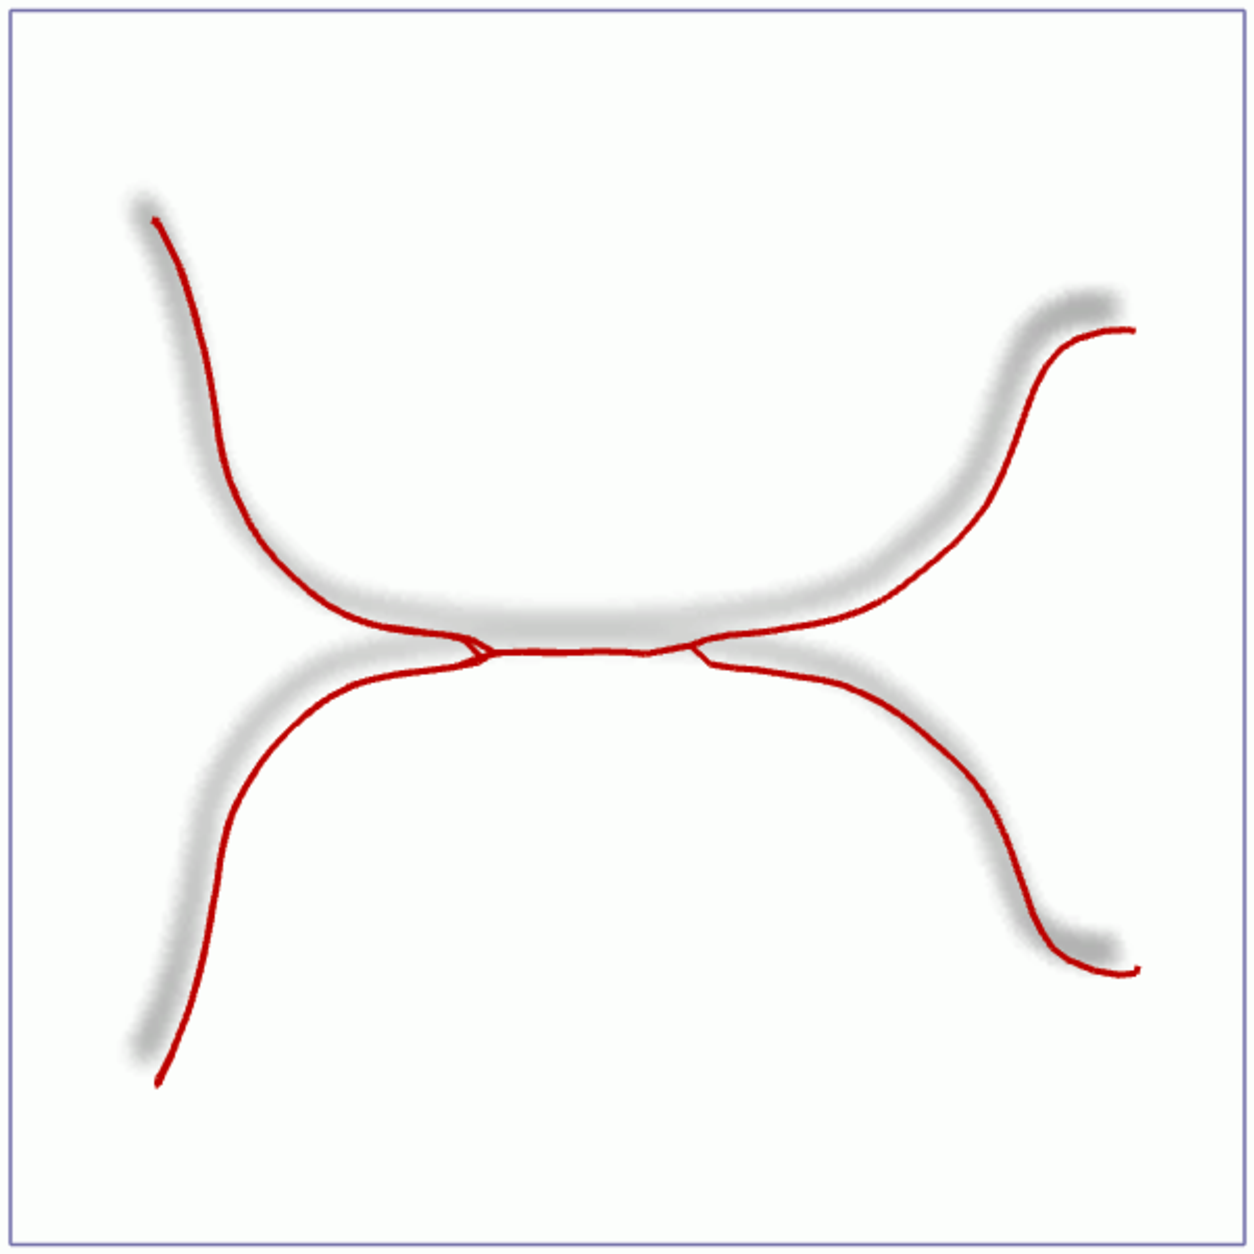
\includegraphics[align=c,width=0.2\columnwidth]{fig10d} &
		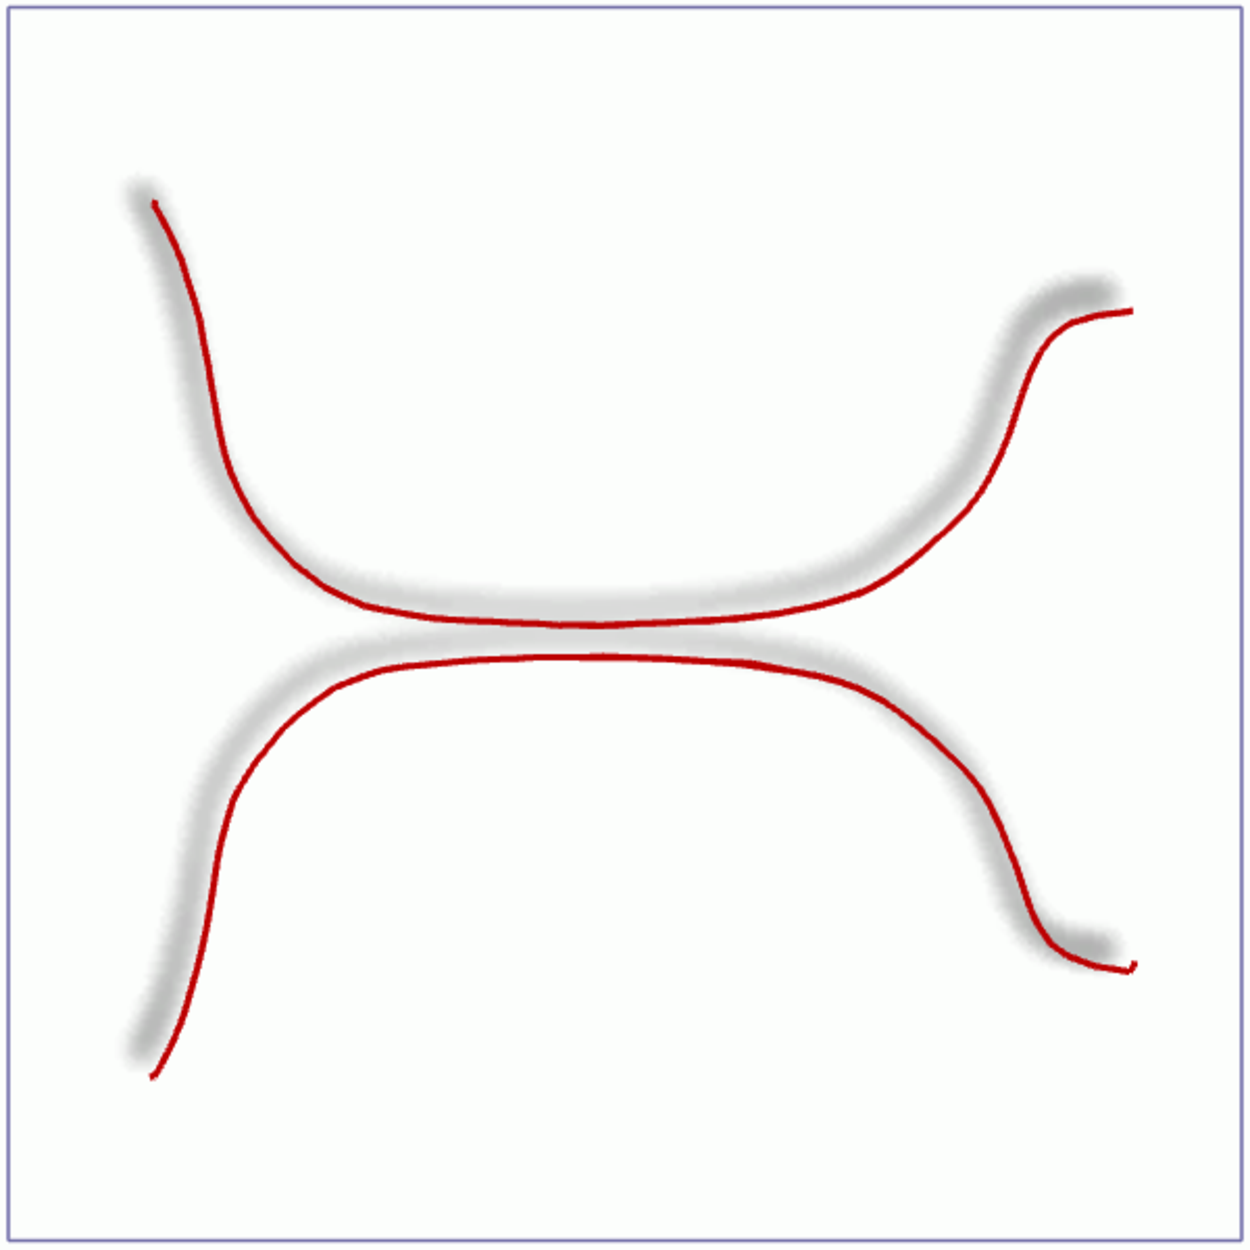
\includegraphics[align=c,width=0.2\columnwidth]{fig10e} &
		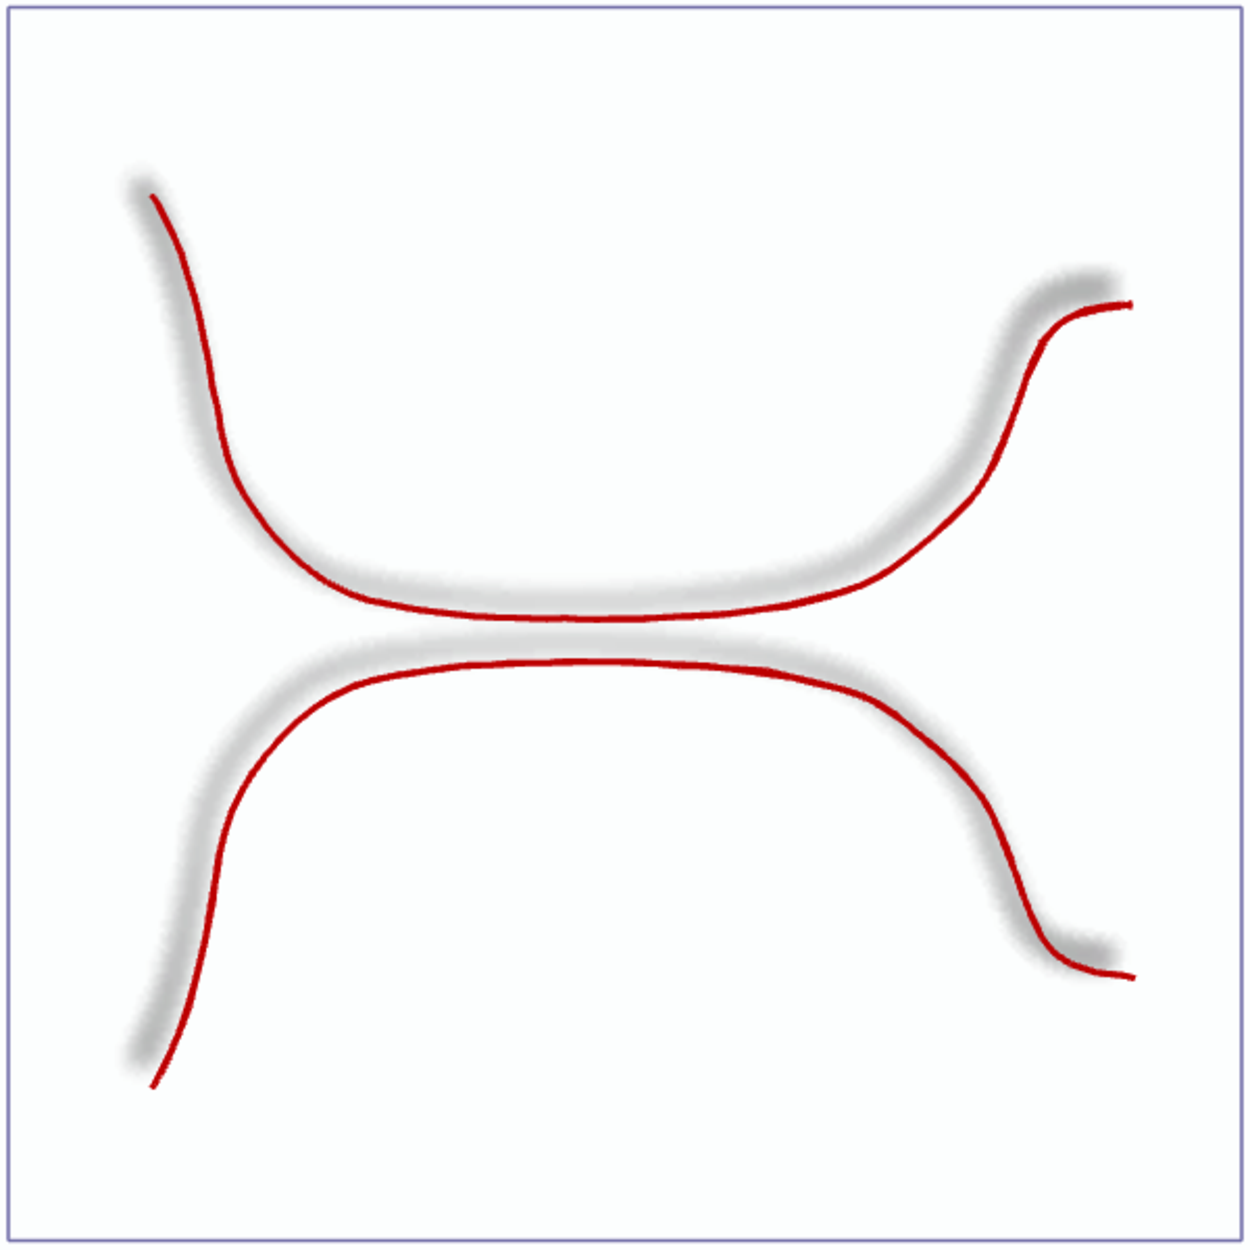
\includegraphics[align=c,width=0.2\columnwidth]{fig10f} \\
		GPS: &
		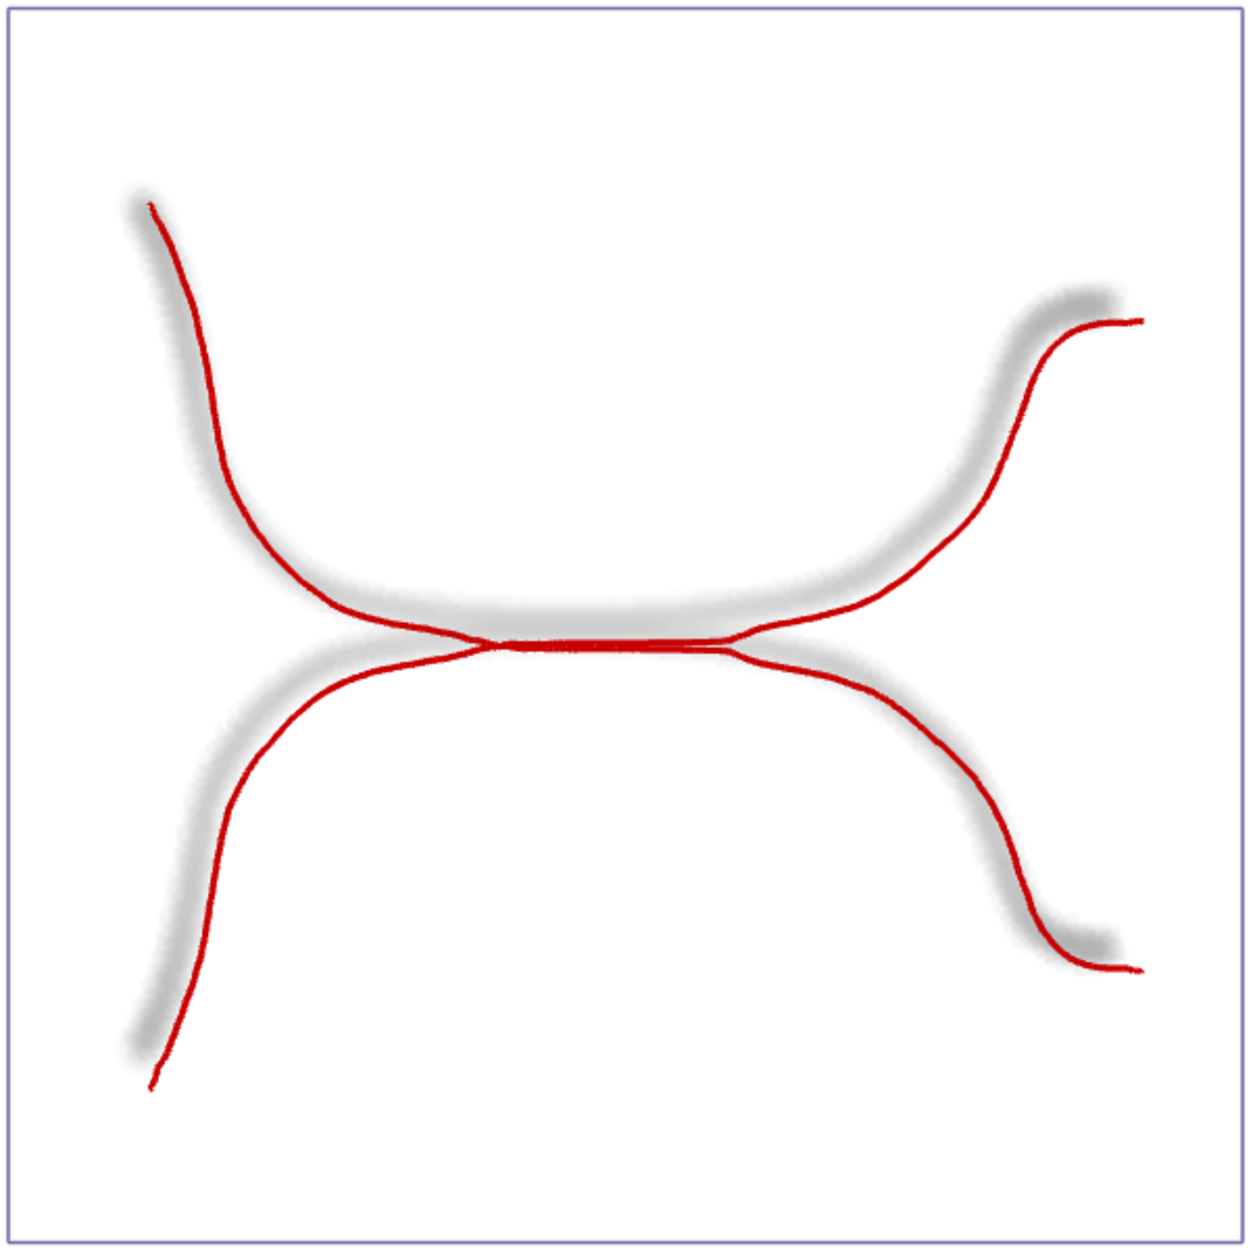
\includegraphics[align=c,width=0.2\columnwidth]{fig10g} &
		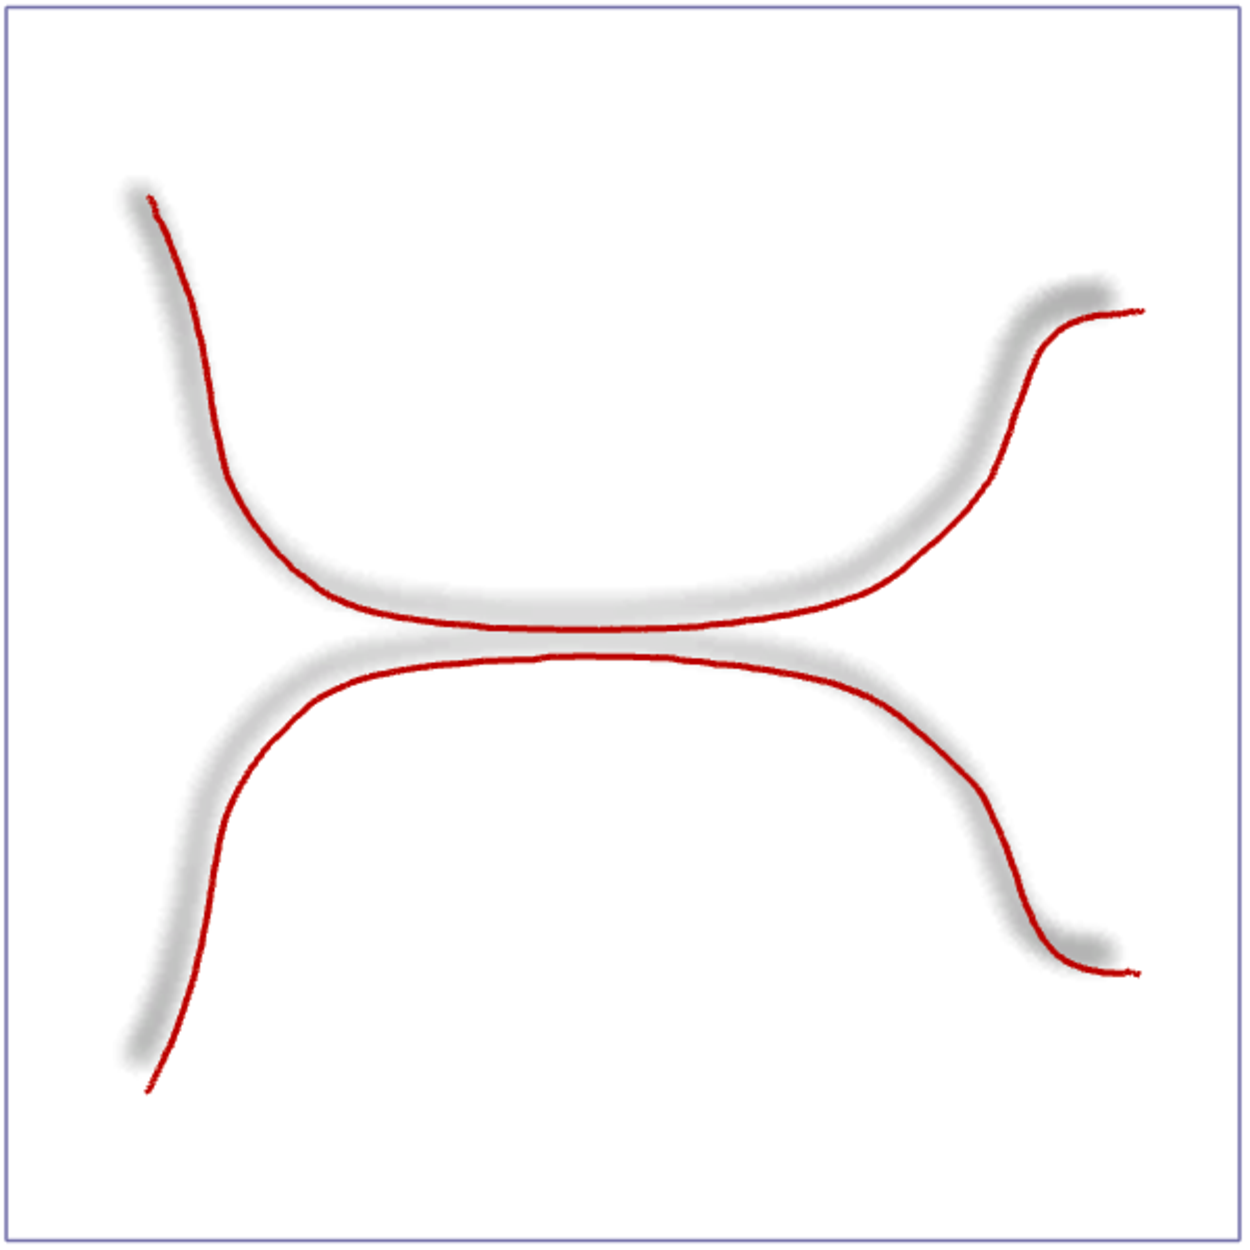
\includegraphics[align=c,width=0.2\columnwidth]{fig10h} &
		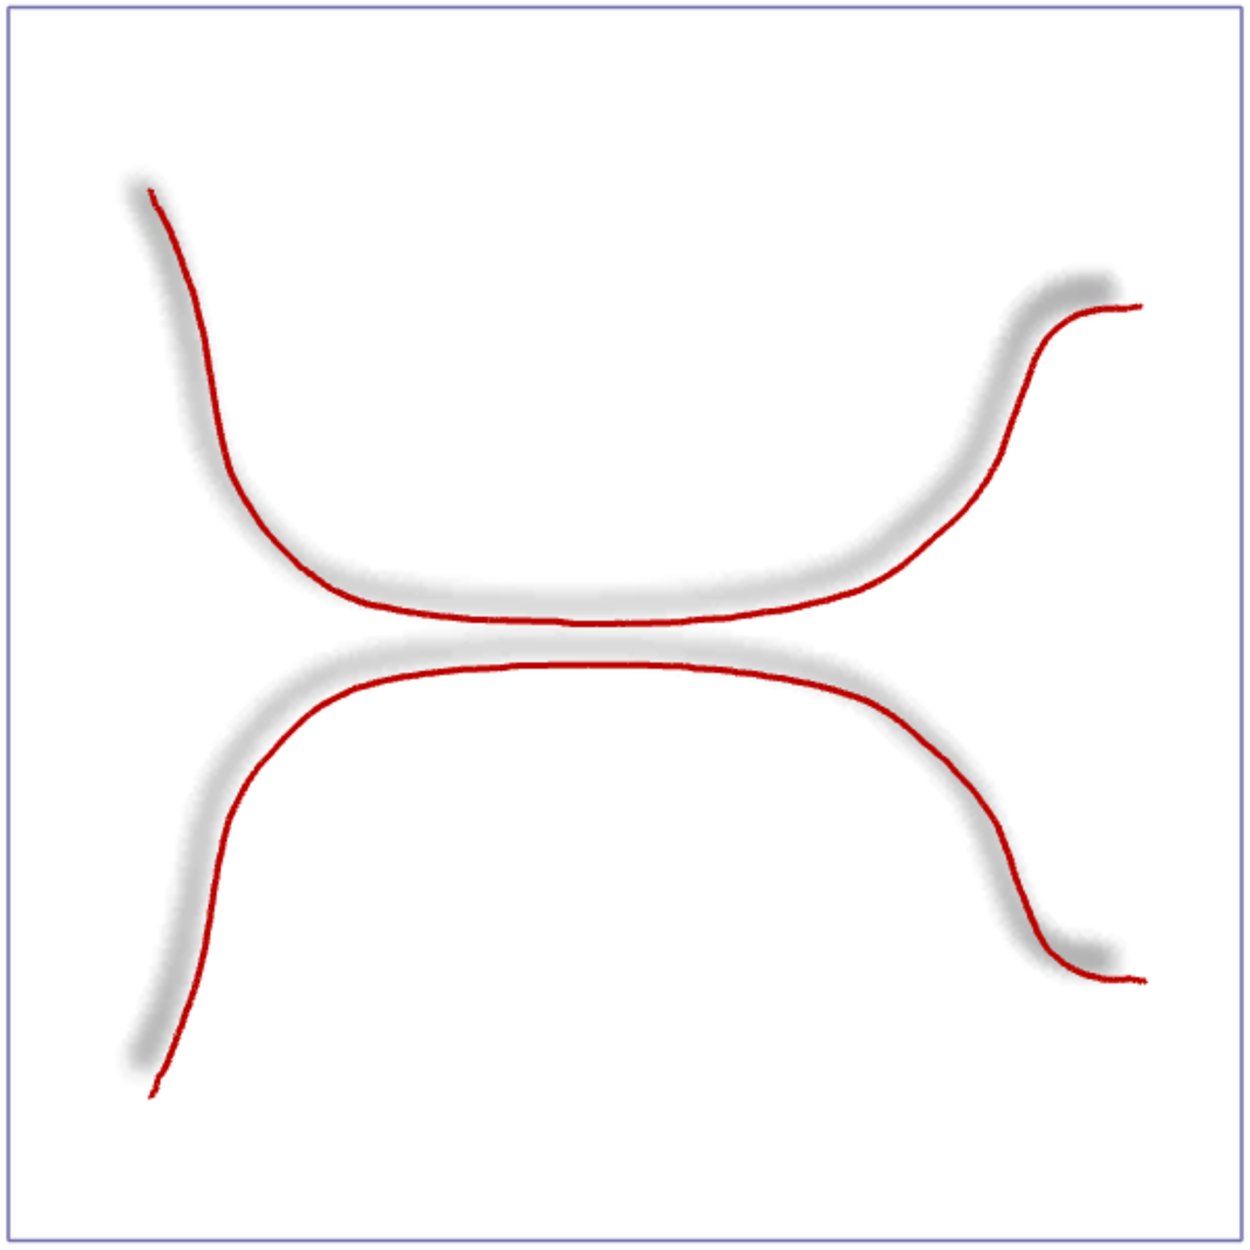
\includegraphics[align=c,width=0.2\columnwidth]{fig10i} \\
		APP2: &
		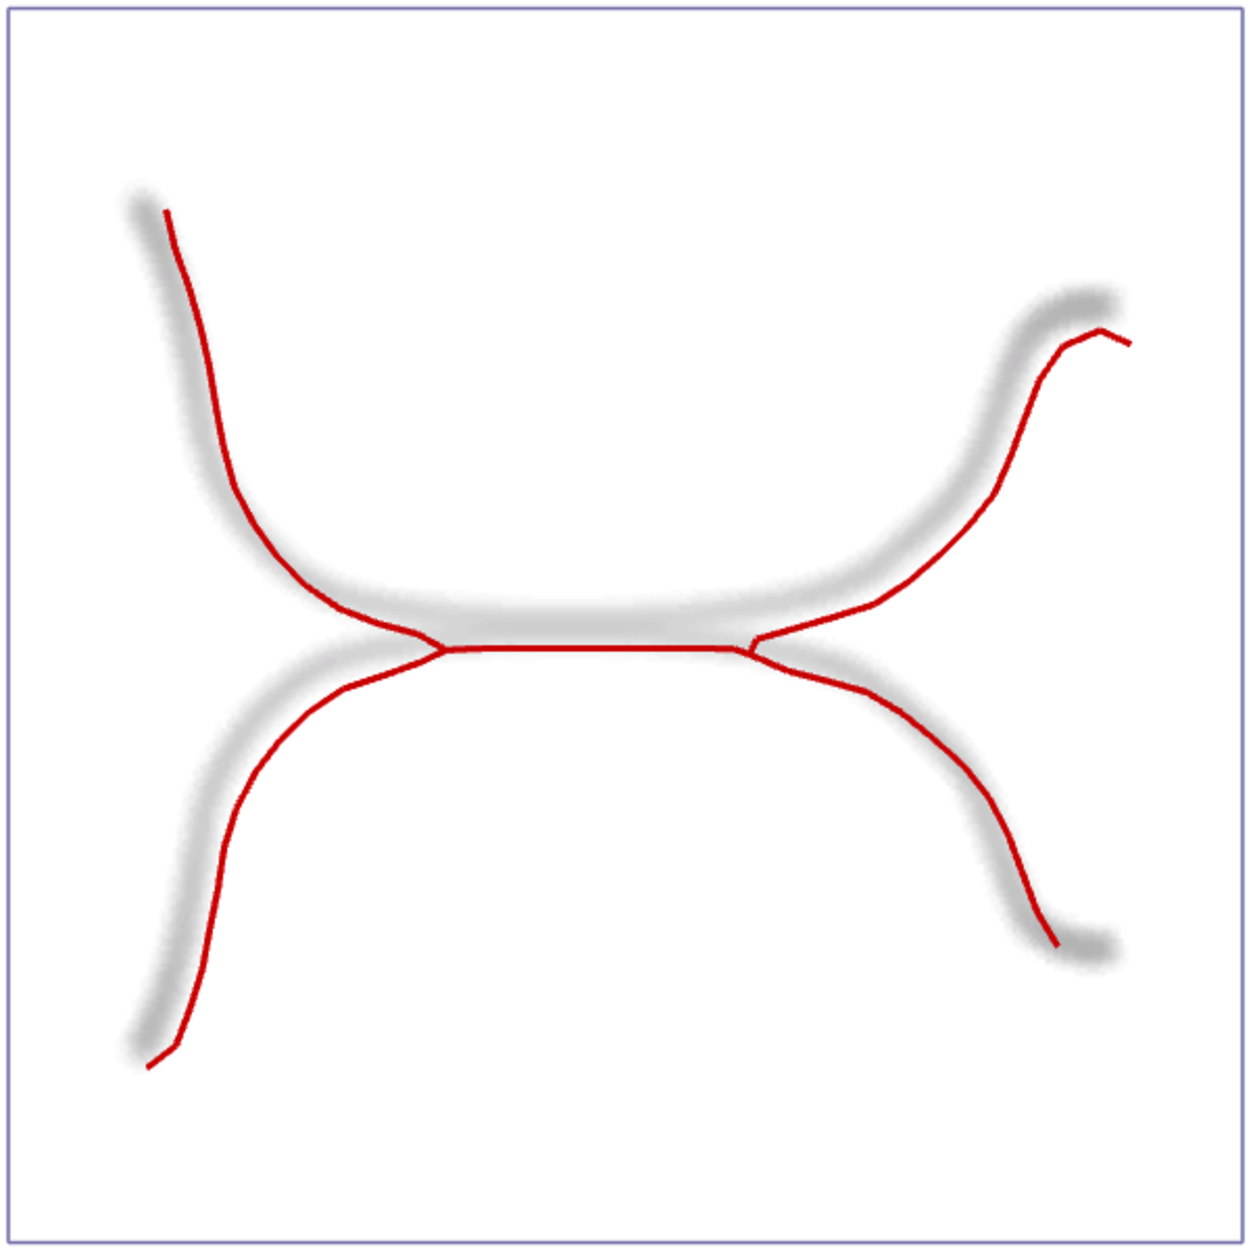
\includegraphics[align=c,width=0.2\columnwidth]{fig10j} &
		\includegraphics[align=c,width=0.2\columnwidth]{fig10k} &
		\includegraphics[align=c,width=0.2\columnwidth]{fig10l} \\
		MST: &
		\includegraphics[align=c,width=0.2\columnwidth]{fig10m} &
		\includegraphics[align=c,width=0.2\columnwidth]{fig10n} &
		\includegraphics[align=c,width=0.2\columnwidth]{fig10p} \\
	\end{tabular}
	\caption{Ability of the tested methods to separate two fibers of similar intensity and scale running closely in parallel. The examples show cases with gradually increasing distance between the fibers: overlap (left column), just separated (middle column), and clearly separated (right column). The tracing results of PHD, GPS, APP2, MST are overlaid (with slight offset) in red color.}
	\label{ch3_fig10}
\end{figure}

\begin{figure}%[!t]
	\centering
	\begin{tabular}{c@{\hspace{0.02\columnwidth}}c@{\hspace{0.02\columnwidth}}c@{\hspace{0.02\columnwidth}}c}
		%\multicolumn{4}{c}{\includegraphics[align=c,width=0.2\columnwidth]{./fig/test2d.compare/i}}\\
		Case: &
		\includegraphics[align=c,width=0.15\columnwidth]{fig11a} &
		\includegraphics[align=c,width=0.15\columnwidth]{fig11b} &
		\includegraphics[align=c,width=0.15\columnwidth]{fig11c}\\
		PHD: &
		\includegraphics[align=c,width=0.2\columnwidth]{fig11d} &
		\includegraphics[align=c,width=0.2\columnwidth]{fig11e} &
		\includegraphics[align=c,width=0.2\columnwidth]{fig11f} \\
		GPS: &
		\includegraphics[align=c,width=0.2\columnwidth]{fig11g} &
		\includegraphics[align=c,width=0.2\columnwidth]{fig11h} &
		\includegraphics[align=c,width=0.2\columnwidth]{fig11i} \\
		APP2: &
		\includegraphics[align=c,width=0.2\columnwidth]{fig11j} &
		\includegraphics[align=c,width=0.2\columnwidth]{fig11k} &
		\includegraphics[align=c,width=0.2\columnwidth]{fig11l} \\
		MST: &
		\includegraphics[align=c,width=0.2\columnwidth]{fig11m} &
		\includegraphics[align=c,width=0.2\columnwidth]{fig11n} &
		\includegraphics[align=c,width=0.2\columnwidth]{fig11p} \\
	\end{tabular}
	\caption{Ability of the tested methods to separate three fibers with different intensity and scale running closely in parallel. The examples show cases with gradually increasing distance between the fibers: overlap (left column), just separated (middle column), and clearly separated (right column). The tracing results of PHD, GPS, APP2, MST are overlaid (with slight offset) in red color.}
	\label{ch3_fig11}
\end{figure}

In terms of computational efficiency it turned out difficult to directly compare the methods. This was mainly due to the use of different programming languages (Java versus C++) and the varying efficiencies of underlying software libraries used on the different operating systems which were considered and used for the computation (Linux Ubuntu and Mac OS). Moreover further observations suggest that the absolute as well as the relative execution times of the different methods varied widely depending on the image content. Generally, APP2 method was found to be the fastest (on the order of seconds per image), and PHD up to about one order of magnitude slower, while GPS and MST were either slower or faster than PHD depending on the configuration. NCT is ignored here for mentioned reasons. From these observations it is possible to draw a conclusion that the efficiency of showcased method is comparable to the state of the art.

\begin{figure}
	\centering
	\begin{tabular}{c@{\hspace{0.02\columnwidth}}c@{\hspace{0.02\columnwidth}}c}
		\includegraphics[width=0.31\columnwidth]{fig12a_embedded} &
		\includegraphics[width=0.31\columnwidth]{fig12b_embedded} & 
		\includegraphics[width=0.31\columnwidth]{fig12c_embedded} \\
		\includegraphics[width=0.31\columnwidth]{fig12d_embedded} &
		\includegraphics[width=0.31\columnwidth]{fig12e_embedded} &
		\includegraphics[width=0.31\columnwidth]{fig12f_embedded} \\
	\end{tabular}
	\caption{Performance comparison of the method with several other methods on the NCL1A data set. For each method and each measure, the plotted box indicates the 25-75 percentile, the horizontal bar indicates the median score, and the whiskers and outliers are drawn using the default settings of R.}
	\label{ch3_fig12}
\end{figure}

\section{Conclusions}
\label{ch3:sec:conclusions}
A new method for tracing the branch centerlines of neurons based on Bayesian multi-object tracking using probability hypothesis density (PHD) filtering was presented. The method is able to simultaneously trace out multiple neuron structures in a probabilistic fashion so that the same neuron segments may be covered multiple times and are thus supported by more evidence. PHD filtering solves the computational problems of direct Bayesian multi-object tracking and allows convenient handling of bifurcations and terminations during the tracing process by modeling of spawned objects and observation clutter. The results of experiments on various fluorescence microscopy image data sets of real neurons showed that the proposed method performs comparably or better than alternative state-of-the-art neuron tracing methods.

The current version of the proposed method is initialized with seed points sampled from the local maxima (from highest to lowest) of the tubularity filter response. This is a rather rudimentary approach that may sometimes result in missed branches (false negatives). Ideally, seeds should be strategically distributed so that they cover as many branches of the neuron structure as possible while avoiding background artifacts, and this is an important topic for further research. In addition, the current mechanism responsible for trace termination, based on the clutter term of the PHD filter, relies strongly on the tubularity score and thus is sensitive to local interruptions in neuron staining. This could be remedied by using a better tubularity filter and/or refining the clutter model. Thus, the future work would involve further study over the possibility of further improvements achieved using different transition and observations models. One of the future aims is also to extend the method to perform local branch radius estimation during tracing in order to obtain complete neuron reconstructions.

Software implementing the proposed neuron tracing method was written in the Java programming language as a plugin for the ImageJ platform. Source code is freely available for non-commercial use at \url{https://bitbucket.org/miroslavradojevic/phd}.
